\documentclass[10pt,a4paper]{article}

% --- Page geometry --------------------------------------------------------
\usepackage[a4paper, top=2.0cm, bottom=2.0cm, left=2.6cm, right=2.6cm]{geometry}

% --- Math, symbols, theorems ---------------------------------------------
\usepackage{amsmath,amssymb,amsthm,mathtools,bm}
\usepackage{thmtools}

% --- Graphics, tables, floats --------------------------------------------
\usepackage{graphicx}
\usepackage{booktabs}
\usepackage{caption}
\captionsetup{font=small,labelfont=bf,labelsep=period}
\usepackage{subcaption}
\usepackage{float}
\usepackage{array}

% Float placement. The defaults reserve so much of a page for text that a
% figure or table which does not fit in the remaining space is deferred and
% the rest of the page is left blank. These are the conventional relaxations:
% allow a float to occupy more of a page, and require less text alongside it.
\renewcommand{\topfraction}{0.92}
\renewcommand{\bottomfraction}{0.75}
\renewcommand{\textfraction}{0.06}
\renewcommand{\floatpagefraction}{0.75}
% Pages holding only floats start at the top instead of spreading the floats apart.
\makeatletter
\setlength{\@fptop}{0pt}
\setlength{\@fpsep}{14pt plus 4pt}
\setlength{\@fpbot}{0pt plus 1fil}
\makeatother
\setcounter{topnumber}{3}
\setcounter{bottomnumber}{2}
\setcounter{totalnumber}{4}

% --- Bibliography & references -------------------------------------------
\usepackage[numbers,sort&compress,square]{natbib}
\usepackage[svgnames]{xcolor}
\usepackage[hyperfootnotes=false]{hyperref}
\hypersetup{colorlinks=true, citecolor=black, linkcolor=black, urlcolor=black,
  pdfauthor={Gregor Albiez},
  pdftitle={Same Formula, Different Signal: Funding-Rate Censoring and Regime Dynamics in Decentralised Perpetual Futures},
  pdfsubject={Funding-rate censoring and regime dynamics in perpetual futures},
  pdfkeywords={funding rates; censoring; perpetual futures; regime switching; hidden Markov models; Hyperliquid; Binance; Bybit; Hamilton filter}}

% --- Typography & spacing ------------------------------------------------
\usepackage[protrusion=true,expansion=false]{microtype}
\usepackage{titling}
\usepackage{titlesec}
\titleformat{\section}{\large\bfseries}{\thesection}{0.7em}{}
\titleformat{\subsection}{\normalsize\bfseries}{\thesubsection}{0.6em}{}
\setlength{\parskip}{4pt}
\setlength{\parindent}{16pt}

% --- Macros --------------------------------------------------------------
\newcommand{\R}{\mathbb{R}}
\newcommand{\E}{\mathbb{E}}
\newcommand{\Prob}{\mathbb{P}}
\newcommand{\Var}{\operatorname{Var}}
\newcommand{\HMM}{\textsc{hmm}}
\newcommand{\MSAR}{\textsc{ms-ar}}
\newcommand{\given}{\mid}
\newcommand{\Filt}{\mathcal{F}}

\title{\Large\bfseries Same Formula, Different Signal:\\[0.3em]
       \large Funding-Rate Censoring and Regime Dynamics\\ in Decentralised Perpetual Futures}
\author{Gregor Albiez\thanks{MSc Finance. Email: \href{mailto:gregor.albiez@students.fhnw.ch}{\nolinkurl{gregor.albiez@students.fhnw.ch}}. GitHub: \href{https://github.com/gelatotrade}{gelatotrade}.}\\[0.45em]
  \normalsize School of Business, University of Applied Sciences and Arts\\
  \normalsize Northwestern Switzerland (FHNW), Basel}
\date{October 2026}

\begin{document}
\maketitle

\begin{abstract}
\noindent Hyperliquid, Binance and Bybit set perpetual funding by the same rule, which pays exactly an interest floor of $0.01\%$ per eight hours whenever the premium lies inside a $10$ bp band. Over 2 October 2025 to 28 April 2026 the same formula sends different signals: $46.0\%$ of Hyperliquid's $5{,}001$ hourly settlements sit exactly on the floor, and $48.4\%$ at the exchanges' settlement hours, against $5.9\%$ on Binance and $7.7\%$ on Bybit. The cause is where the premiums sit --- the exchanges' just below the band, Hyperliquid's across its lower edge with a long tail into it --- and the gap persists over the five months that follow, $51.7\%$ against $10.9\%$ and $7.9\%$. Hyperliquid's headline rate is censored about half the time; its premium, not its rate, carries the signal.

Fitted to that premium, a two-state Markov-switching AR(1) reverts in $36$ hours when calm and $3.2$ under stress, a ratio of $11$ with a $95\%$ interval of $[3, 19]$. One hour carries its significance. Replacing the crash hour of 10 October 2025 with the next largest observation leaves $3.0$ on an interval covering unity, only one of fourteen rolling windows lies significantly above unity, and the five months after the sample reverse the ordering, at $0.23$, its $95\%$ interval ending at $0.49$. The premium likelihood also has a dominant basin that is not its maximum: $24$ of $40$ estimations settle there and report a ratio of $25$. On returns, a three-state Gaussian \HMM\ separates hourly volatility into $14.6\%$, $33.3\%$ and $88.4\%$ annualised states, and the estimated probability of a direct exit from the high state to the low is zero, with a $95\%$ bound of $0.3\%$ per hour. All results are descriptive.

\noindent\textbf{Keywords:} funding rates; censoring; perpetual futures; regime switching; hidden Markov models; Hyperliquid; Binance; Bybit; Hamilton filter.

\noindent\textbf{JEL:} C22, C58, G12, G13.
\end{abstract}

% =========================================================================
\newpage
\section{Introduction}\label{sec:intro}

Perpetual futures dominate cryptocurrency derivatives, with daily volumes above \$100 billion in 2022, two to three times spot turnover \citep{he2022perp}, and decentralised venues, Hyperliquid foremost, have become structurally significant. Having no expiry, a perpetual is tied to its index by a recurring funding payment between longs and shorts, set from an averaged premium \citep{ackerer2024,hyperliquid_funding_docs}. Hyperliquid, Binance and Bybit compute it with the same rule, and inside a band of premia that rule pays exactly the interest rate, so the published rate stops moving with the market (Figure~\ref{fig:censoring}a). How often that happens decides whether the headline rate can be read as a signal at all.

Funding has a literature on the carry and basis side. \citet{schmeling2025crypto} read crypto carry as compensation for the limits to arbitrage that anchor perpetuals to spot, \citet{makarov2020trading} document the frictions segmenting these markets, \citet{alexander2020bitmex} study price discovery on the first large perpetual venue, \citet{werapun2026funding} compare funding arbitrage across centralised and decentralised exchanges, and \citet{hugonnier2025clamp} model perpetual pricing with the clamp explicitly and report a bimodal distribution of perpetual prices on Binance that they attribute, tentatively, to it. Regime detection in Bitcoin returns is well studied \citep{giudici2020,koki2022bitcoin,machimbo2025}: volatility clusters and breaks \citep{ardia2019}, tails are heavy \citep{koki2022bitcoin} and activity moves with returns \citep{koutmos2018}, which the Markov-switching framework of \citet{hamilton1989} and the hidden Markov machinery of \citet{rabiner1989} capture with a few latent states. \citet{zhivkov2026temporal} apply Bai--Perron tests to rolling cross-exchange integration statistics across 26 venues and find no discrete structural breaks, and a companion paper documents a two-tiered funding market \citep{zhivkov2026funding}; their object is an integration statistic tested for breaks, ours a latent-state decomposition of one venue, but a reader should know that a study on overlapping data finds no breaks where we find states.

We make three contributions, all descriptive and in-sample. First, a measurement: one rule pins the headline rate to the floor in $46.0\%$ of Hyperliquid's hours and in $5.9\%$ and $7.7\%$ of Binance's and Bybit's settlements, because the exchanges' premiums sit just below the band while Hyperliquid's straddles its edge (Section~\ref{ssec:clamp}). Headline funding compared across venues therefore mixes censoring with differences in premium, and on Hyperliquid the premium is the object to model. Second, a joint regime description of the return and premium processes of one decentralised perpetual, whereas the regime literature rests almost entirely on spot prices at centralised venues: three hourly volatility states whose direct move from high to low is estimated at zero, on the boundary, and bounded below $0.3\%$ per hour (Section~\ref{sec:returns}), and a premium whose apparent asymmetry in mean reversion belongs to a single episode, the crash hour of 10 October 2025 (Section~\ref{sec:funding}). Third, a caution that travels: the premium likelihood is multi-modal, and its most frequent optimum, which a single estimation reports reliably enough to look converged, is not its maximum (Figure~\ref{fig:optima}). Figure~\ref{fig:windows} maps the windows and data behind every result.

% =========================================================================
\section{Econometric Framework}\label{sec:framework}

\subsection{Gaussian Hidden Markov Model on Returns}\label{ssec:hmm}

Let $r_t$ be the hourly log-return and $S_t\in\{1,\dots,K\}$ a latent state. The Gaussian \HMM\ has the joint law
\begin{equation}\label{eq:hmm-joint}
  \Prob(r_{1:T},S_{1:T}\given\theta) \;=\; \pi_{S_1}\, b_{S_1}(r_1)\,\prod_{t=2}^{T} A_{S_{t-1},S_t}\, b_{S_t}(r_t),
\end{equation}
with $\pi_i = \Prob(S_1=i)$, $A_{ij}=\Prob(S_t=j\given S_{t-1}=i)$ and emission $b_k(r) = \varphi(r;\mu_k,\sigma_k^2)$. The \emph{filtered} posterior $\Prob(S_t=k\given\Filt_t)$, with $\Filt_t = \sigma(r_{1:t})$, uses only the past and is the one admissible for real-time use; the \emph{smoothed} posterior $\Prob(S_t=k\given\Filt_T)$ conditions on the whole sample and serves only as an in-sample diagnostic. We estimate by Baum--Welch from eight random starts, keep the highest likelihood, and order states by $\hat\sigma_k$ ascending --- low, moderate and high volatility --- because the means are too close to order by; Appendix~\ref{app:estimation} gives the recursions and the case against a $\mu$-ascending rule.

Model selection uses BIC over $K\in\{2,3\}$, with $K^2+2K-1$ free parameters, $7$ and $14$; Section~\ref{ssec:robust} adds $K{=}4$ and $5$. A likelihood-ratio test is not available: under $K{=}2$ the third state's parameters are unidentified and the statistic has no $\chi^2$ limit \citep{davies1987,hansen1992,cho2007}, so we read the criteria as evidence, not as tests at a nominal size. Penalised-likelihood order estimation is consistent for mixtures and for finite-alphabet hidden Markov models \citep{keribin2000,gassiat2003}.

\subsection{Markov-Switching AR(1) for the Funding Premium}\label{ssec:msar}

For the premium $y_t$ in basis points we use the mean-adjusted two-state form of \citet{hamilton1989},
\begin{equation}\label{eq:msar}
  y_t - \mu_{S_t} \;=\; \phi_{S_t}\bigl(y_{t-1} - \mu_{S_{t-1}}\bigr) + \sigma_{S_t}\,\varepsilon_t,\qquad \varepsilon_t \stackrel{\text{iid}}{\sim} \mathcal{N}(0,1),
\end{equation}
in which $\mu_k$ is the regime \emph{level}, not an intercept, all of $(\mu_k,\phi_k,\sigma_k)$ switch, and the likelihood conditions on the pair $(S_t, S_{t-1})$. The half-life
\begin{equation}\label{eq:halflife}
  \tau_k = \frac{\ln 0.5}{\ln |\phi_k|}
\end{equation}
says in hours how long half of a premium dislocation takes to decay within regime $k$. We estimate by maximum likelihood with the Hamilton filter and the smoother of \citet{kim1994dynamic} as implemented in \texttt{statsmodels} and, because the likelihood is multi-modal (Section~\ref{ssec:msar-robust}), always from 40 estimations of 40 random initialisations each, reporting the highest terminal log-likelihood.

\subsection{Conditional Moments}\label{ssec:cond-moments}

With the predicted state distribution $\tilde p_{j,t} \equiv \Prob(S_{t+1}=j\given\Filt_t) = \sum_k \Prob(S_t=k\given\Filt_t)\,A_{kj}$, the one-step conditional mean and variance of returns are
\begin{equation}\label{eq:cond-mean}
  \E[r_{t+1}\given\Filt_t] \;=\; \sum_{j=1}^K \tilde p_{j,t}\, \mu_j \equiv \bar\mu_t,
\end{equation}
\begin{equation}\label{eq:cond-var}
  \Var(r_{t+1}\given\Filt_t) \;=\; \underbrace{\sum_j \tilde p_{j,t}\,\sigma_j^2}_{\text{within-regime}} \;+\; \underbrace{\sum_j \tilde p_{j,t}\,(\mu_j - \bar\mu_t)^2}_{\text{between-regime}},
\end{equation}
the second term being the variance that regime uncertainty itself adds, a feature absent from single-regime stochastic-volatility models.

% =========================================================================
\section{Data and Funding Mechanics}\label{sec:data}

\subsection{Sample Construction}

For the BTC perpetual we take Hyperliquid's hourly candles of traded prices and its hourly funding observations from the public endpoints \texttt{candleSnapshot} and \texttt{fundingHistory}, floored to the hour and inner-joined: $T = 5{,}001$ observations from 2 October 2025 00:00 UTC to 28 April 2026 08:00 UTC, retrieved on 28 April 2026. For Section~\ref{ssec:clamp} we add, retrieved on 6 October 2026, the funding histories and hourly premium index of the Binance and Bybit BTCUSDT perpetuals from 1 October 2025 to 30 September 2026. Beyond the estimation window, every funding series runs to the settlement stamped 1 October 2026 00:00 UTC, which pays for the final hours of 30 September. Figure~\ref{fig:windows} shows the windows and which series survive at which resolution.

The data set the window. \texttt{fundingHistory} keeps a contract's whole history, and returns an unbroken hourly BTC series from June 2023; \texttt{candleSnapshot} serves only the most recent $5{,}000$ or so candles at each interval, so it reaches some 208 days back at hourly resolution, 417 at two-hourly and 833 at four-hourly. The premium series is therefore replicable and extensible in both directions; the hourly return series is not, its first two months having left the hourly window before the panel was archived. Two-hourly candles re-retrieved in August 2026 agree bit for bit with the surviving hourly panel aggregated to two hours on all $1{,}753$ overlapping bars; they bound the return extrema of Table~\ref{tab:summary} and check the state structure in Section~\ref{ssec:robust}. Both models use the common $5{,}001$-hour window, which contains the local high of \$126{,}101 and the February 2026 trough of \$62{,}883.

Returns are $r_t = \ln(p_t/p_{t-1})$ on the last traded price of hour $t$, not the mark price, in basis points; funding is in basis points per hour and the premium in 8-hour-equivalent basis points. Annualisation uses $\sqrt{24\cdot 365}$ for volatility and $24\cdot 365$ for funding.

\begin{figure}[!htbp]
  \centering
  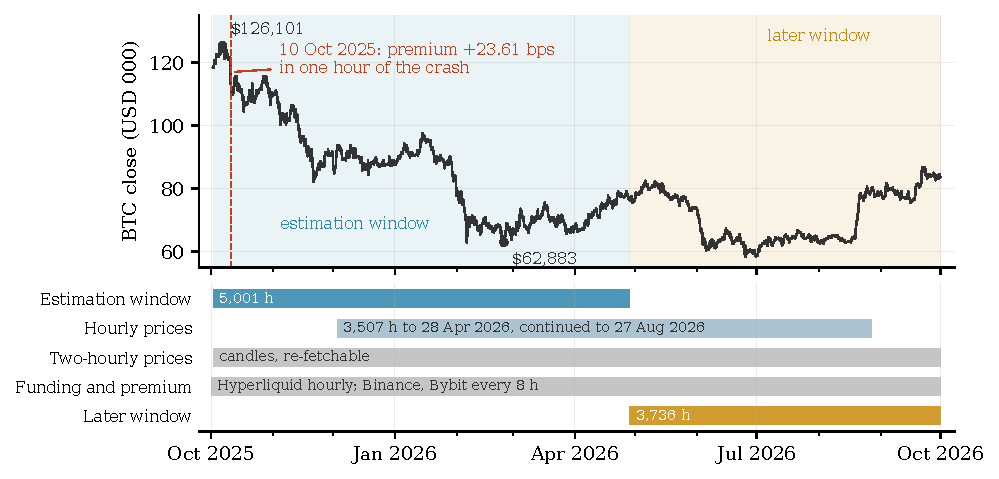
\includegraphics[width=\textwidth]{figures/fig5_windows.pdf}
  \caption{Windows and data. \textbf{Top}: BTC two-hourly close, the estimation window (2 October 2025 -- 28 April 2026) and the later window (28 April -- 30 September 2026) shaded, with the price extremes of Table~\ref{tab:summary} and the premium's maximum hour marked. \textbf{Bottom}: the windows and the series the replication package ships; hourly prices survive only from 3 December 2025.}
  \label{fig:windows}
\end{figure}

\begin{table}[!htbp]
  \centering
  \caption{Summary statistics for hourly observations on Hyperliquid BTC perpetual, 2 Oct 2025 -- 28 Apr 2026 ($T = 5{,}001$).}
  \label{tab:summary}
  \begin{tabular}{lrrrrrr}
    \toprule
    Series & Mean & Std. dev. & Min & Median & Max & Skew \\
    \midrule
    Log-return (bps/h)        & $-0.87$ & $50.92$ & \textdagger & $-0.27$ & \textdagger & $-0.21$ \\
    Funding rate (bps/h)      & $0.059$ & $0.103$ & $-0.694$ & $0.111$ & $2.327$ & $+0.94$ \\
    Premium (bps)             & $-3.15$ & $2.87$ & $-10.55$ & $-4.11$ & $23.61$ & $+1.71$ \\
    Closing price (USD)       & $86{,}314$ & $15{,}988$ & $62{,}883$ & $87{,}678$ & $126{,}101$ & --- \\
    \bottomrule
  \end{tabular}

  \smallskip
  \begin{minipage}{\linewidth}\footnotesize \textdagger\ Withheld. The values recorded at retrieval, $-3{,}800$ and $+3{,}421$ bps/h, are inconsistent with the standard deviation beside them: the two alone would contribute twice the sample's sum of squared deviations. Mean and standard deviation are reproduced by the fitted mixture of Table~\ref{tab:regime-params}, $-0.87$ and $50.95$ bps/h, so the extrema are in error (median and skewness of a dependent sample need not match the mixture's). The two-hourly candles bound every hourly move by the high--low range of its two-hour bar, at most $1{,}498$ bps ($14.98\%$, on 10 October 2025), excluding the recorded values by factors of $2.3$ and $2.5$. On the hourly sub-period of Section~\ref{ssec:robust} the realised range is $[-367.5, +336.7]$ bps/h.\end{minipage}
\end{table}

\subsection{The Funding Formula and the Clamp Artifact}\label{ssec:clamp}

Hyperliquid's documentation specifies the 8-hour-equivalent funding rate as
\begin{equation}\label{eq:hl-funding}
  F_t \;=\; \bar P_t + \operatorname{clamp}\bigl(r - \bar P_t,\, -5 \cdot 10^{-4},\, +5 \cdot 10^{-4}\bigr),
\end{equation}
with $\bar P_t$ the premium index averaged over the preceding hour, $r = 10^{-4}$ the interest rate per eight hours and $\operatorname{clamp}(x,a,b) = \max(a,\min(b,x))$; the hourly payment is $F_t / 8$ \citep{hyperliquid_funding_docs}. Binance and Bybit use the same $0.01\%$ interest and $\pm 0.05\%$ clamp \citep{binance_funding_docs,bybit_funding_docs}, with which Hyperliquid states its rule is designed to be consistent; \citet{kim2025funding} study the design problem such a rule solves. The venues differ in schedule --- hourly against every eight hours --- and in how each builds its premium index, from its own index price and impact size, and averages it over its own settlement interval.

Figure~\ref{fig:censoring}(a) draws the rule. Whenever $\bar P_t \in (-4, +6)$ bps --- a band centred on $+1$ bp, not on zero --- the clamp is the identity and $F_t = r$: the hourly rate is exactly $0.125$ bps/h, which we call the interest floor, although rates fall below it whenever the premium lies below the band. Hyperliquid's premium has a mean of $-3.15$ bps, just inside the band's lower edge, and $2{,}300$ of $5{,}001$ hours --- $46.0\%$ --- sit exactly on the floor; the count is exact, the floor hours being precisely those with $\bar P_t$ inside the band. The hourly schedule does not cause the share. Read every eighth hour, the series gives $44.2\%$ to $48.4\%$ by phase offset, averaging $46.0\%$; the exchanges' 00, 08 and 16 UTC stamps give the top of that range, but only one point above the hourly share after the window ($52.7\%$ against $51.7\%$, Table~\ref{tab:censoring}), differences of a few points beside a gap of forty. An eight-hour average, with a standard deviation of $2.75$ bps against $2.87$, even lands in the band more often, $48.0\%$ of the time: the schedule multiplies censored payments, not censored observations.

The point mass breaks any Gaussian regime model of $F_t$: an \MSAR\ fitted to the rate returns a degenerate regime with $\hat\sigma^2$ of order $10^{-32}$ pinned to the floor and one ordinary regime with $\hat\phi = 0.81$. We therefore model the premium $\bar P_t$, which \texttt{fundingHistory} publishes beside each rate. The two series point in opposite directions (Table~\ref{tab:summary}): funding averaged $+0.059$ bps/h, about $+5.2\%$ a year, so longs paid shorts, while the premium averaged $-3.15$ bps, the contract trading below its index for much of the sample. In the $46.0\%$ of hours with the premium inside the band the contract paid the floor whatever the positioning, and a reader of the headline rate as positioning would see longs paying over a window in which the contract mostly traded below its index.

\paragraph{Same formula, different signal.} Binance and Bybit settle every eight hours under the same rule, and their funding histories make the comparison exact: a settlement equals the floor exactly when the averaged premium sat inside the band, and any other settlement identifies that premium, as the settlement minus $0.05\%$ below the band or plus $0.05\%$ above it. Over the paper window Binance prints the floor in $37$ of $626$ settlements ($5.9\%$) and Bybit in $48$ ($7.7\%$), against $46.0\%$ on Hyperliquid, which still prints it $48.4\%$ of the time read at the exchanges' 00, 08 and 16 UTC stamps (Figure~\ref{fig:censoring}c, Table~\ref{tab:censoring}). No exchange settlement exceeds the floor; $94.1\%$ of Binance's and $92.3\%$ of Bybit's lie below it. The five months after the window repeat the pattern, $51.7\%$ on Hyperliquid against $10.9\%$ and $7.9\%$.

The premiums explain the difference (Figure~\ref{fig:censoring}b). Recovered from their settlements, the exchanges' premiums are concentrated just below the band, with medians of $-4.75$ and $-4.82$ bps and interquartile ranges of $0.66$ and $0.60$ bp. Hyperliquid's straddles the edge --- median $-4.11$ bps, $52.5\%$ of hours below the band --- with a long tail into the band that lifts its mean to $-3.15$. The censored share is a property of where a venue's premium sits, not of the formula, which is shared, nor of when settlements are sampled, although how each venue averages its premium may contribute: an eight-hour average narrows a distribution whose mean lies below the band and so lowers the share inside it. Funding-arbitrage studies rightly use the cash flow \citep{werapun2026funding}; read as positioning, headline funding compared across venues sets a series censored half the time against ones that rarely are, and the premiums, which the rule does not censor, are the better basis, though their windows and indices differ.

\begin{figure}[!htbp]
  \centering
  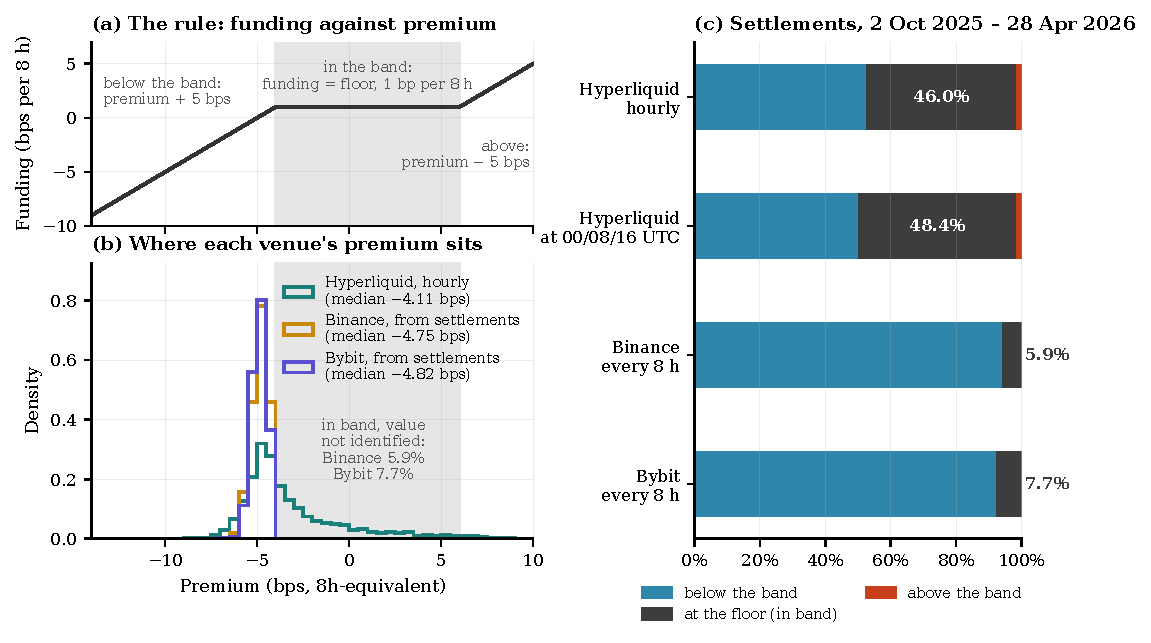
\includegraphics[width=\textwidth]{figures/fig4_censoring_venues.pdf}
  \caption{Funding-rate censoring across venues, BTC perpetuals, 2 October 2025 -- 28 April 2026. \textbf{(a)} The rule~\eqref{eq:hl-funding}: funding per eight hours against the averaged premium; inside the band $(-4, +6)$ bps it pays exactly the floor of $1$ bp. \textbf{(b)} Where each venue's premium sits: Hyperliquid's hourly average premium, and the Binance and Bybit premiums recovered exactly from their settlements. Settlements at the floor say only that the premium lay inside the band and are not drawn, so each exchange's curve integrates to its identified share. \textbf{(c)} Shares of settlements below the band, exactly at the floor, and above it: Hyperliquid hourly and read at 00, 08 and 16 UTC, and the eight-hourly settlements of Binance and Bybit.}
  \label{fig:censoring}
\end{figure}

\begin{table}[!htbp]
  \centering
  \caption{Funding settlements exactly at the interest floor, compared as decimals, per venue and window. \emph{Below}: settlements under the floor, the premium below the band. \emph{Median} and \emph{IQR}: premium in bps, Hyperliquid's hourly average and the exchanges' recovered from settlements; floor settlements rank between those below and above the band, so the quantiles are exact. The second Hyperliquid row reads the hourly series at the exchanges' settlement stamps.}
  \label{tab:censoring}
  \small
  \setlength{\tabcolsep}{4pt}
  % Generated by regime_engine.censoring -- do not edit by hand.
% Settlements exactly at the interest floor, compared as decimals; see
% output/censoring_comparison.json.
\begin{tabular}{llrrrrrrr}
\toprule
 & & \multicolumn{5}{c}{2 Oct 2025 -- 28 Apr 2026} & \multicolumn{2}{c}{28 Apr -- 30 Sep 2026} \\
\cmidrule(lr){3-7}\cmidrule(lr){8-9}
Venue & Settles & $n$ & At floor & Below & Median & IQR & $n$ & At floor \\
\midrule
Hyperliquid & hourly & 5,001 & 46.0\% & 52.5\% & $-$4.11 & [$-$4.93, $-$2.26] & 3,736 & 51.7\% \\
Hyperliquid & at 00/08/16 UTC & 626 & 48.4\% & 50.0\% &  &  & 467 & 52.7\% \\
Binance & every 8 h & 626 & 5.9\% & 94.1\% & $-$4.75 & [$-$5.10, $-$4.44] & 467 & 10.9\% \\
Bybit & every 8 h & 626 & 7.7\% & 92.3\% & $-$4.82 & [$-$5.09, $-$4.49] & 467 & 7.9\% \\
\bottomrule
\end{tabular}

\end{table}

% =========================================================================
\section{Regime Estimation: Returns}\label{sec:returns}

\subsection{Model Selection}\label{ssec:modelsel}

BIC prefers $K{=}3$ to $K{=}2$ by about $217$ points (Table~\ref{tab:modelsel}): the third state's likelihood gain outweighs its seven extra parameters. We read the difference as evidence, not as a test at a nominal size, and attach no Bayes-factor reading to its magnitude \citep{kass1995bayes}.

\begin{table}[!htbp]
  \centering
  \caption{Information criteria for $K\in\{2,3\}$ on $T=5{,}001$ hourly log-returns.}
  \label{tab:modelsel}
  % Manuscript copy. Window: 2 Oct 2025 -- 28 Apr 2026 (T = 5,001) -- the FULL
% sample, which no longer exists at hourly resolution and cannot be refitted.
% Source: the K=3 row is output/summary_FULLSAMPLE_2025-10-02_to_2026-04-28.json
% (return_K3.logL / .BIC). The K=2 row was not archived and cannot be refitted,
% because the full-sample hourly returns are no longer served; it survives only
% here and in the PDF. The corresponding sub-sample comparison, which is
% reproducible, is in output/summary.json under model_selection
% (delta BIC -176.59).
% output/tables/table1_model_selection.tex carries the SAME FILENAME but the
% T = 3,507 sub-sample fit. Do not overwrite this file with it.
\begin{tabular}{lrrrr}
\toprule
$K$ & $\log\mathcal{L}$ & \# params & AIC & BIC \\
\midrule
2 & 20,132.0 & 7 & $-$40,250.0 & $-$40,204.4 \\
3 & 20,270.2 & 14 & $-$40,512.4 & $-$40,421.1 \\
\bottomrule
\end{tabular}

\end{table}

\subsection{Regime Parameters and Geometry}

Table~\ref{tab:regime-params} reports the $K{=}3$ fit. The states separate on volatility and only on volatility: $15.6$, $35.6$ and $94.4$ bps/h, or $14.6\%$, $33.3\%$ and $88.4\%$ annualised, with bootstrap intervals of $[13.6, 15.5]$, $[31.8, 34.9]$ and $[83.0, 94.0]$ per cent that are nowhere near overlapping, and stationary masses of $20$, $60$ and $20\%$. No drift separates from zero: the largest, $\hat\mu_3 = -5.69$ bps/h, has a standard error of $3.28$ and an interval of $[-12.44, +0.27]$, so we do not call the high-volatility state one of negative expected return.

\begin{table}[!htbp]
  \centering
  \caption{Regime parameters of the $K{=}3$ Gaussian \HMM\ on hourly log-returns. Annualised $\sigma$ uses $\sigma\sqrt{24\cdot 365}$; expected duration is $\E[\tau_k] = 1/(1-A_{kk})$. Parenthesised figures are parametric-bootstrap standard errors (Section~\ref{ssec:inference}).}
  \label{tab:regime-params}
  % Manuscript copy. Window: 2 Oct 2025 -- 28 Apr 2026 (T = 5,001) -- the FULL
% sample, not refittable: hourly candles before 3 Dec 2025 are no longer served.
% Point estimates: output/summary_FULLSAMPLE_2025-10-02_to_2026-04-28.json,
%   re-indexed to sigma ascending (that file stores mu-ascending arrays).
% Parenthesised standard errors: output/bootstrap_hmm.json, sigma_ascending block.
% output/tables/table2_regime_params.tex carries the SAME FILENAME but the
% T = 3,507 sub-sample fit and no standard errors. Do not overwrite this file.
\begin{tabular}{lrrrrr}
\toprule
State & $\hat\mu_k$ (bps/h) & $\hat\sigma_k$ (bps/h) & Annualised $\hat\sigma_k$ & $\hat A_{kk}$ & $\mathbb{E}[\tau_k]$ (h) \\
\midrule
1 low      & $0.139$  & $15.55$ & $14.6\%$ & $0.9235$ & $13.1$ \\
           & $(0.62)$ & $(0.52)$ & $(0.49)$ & $(0.0120)$ & $(2.08)$ \\
2 moderate & $0.404$  & $35.57$ & $33.3\%$ & $0.8867$ & $8.8$ \\
           & $(0.78)$ & $(0.87)$ & $(0.82)$ & $(0.0114)$ & $(0.90)$ \\
3 high     & $-5.685$ & $94.42$ & $88.4\%$ & $0.7307$ & $3.7$ \\
           & $(3.28)$ & $(2.97)$ & $(2.78)$ & $(0.0303)$ & $(0.42)$ \\
\bottomrule
\end{tabular}

\end{table}

These are hourly states. Expected durations of $13.1$, $8.8$ and $3.7$ hours imply some $686$ state visits over $5{,}001$ hours, one switch about every seven, and some 270 entries into the high state in seven months: a three-bucket classifier of hourly conditional volatility, not a description of market phases. The fitted chain, with geometric durations of a few hours, does not generate the persistence that \emph{regime} and \emph{crisis} usually connote; that would need duration dependence or time-varying transition probabilities \citep{filardo1994business}.

\paragraph{The transition geometry.}\label{par:funnel} Figure~\ref{fig:transitions} draws the kernel. Exits from the high state route through the moderate one ($\hat A_{32} \approx 0.27$, s.e.\ $0.030$); the direct move to the low state, $\hat A_{31}$, is estimated at exactly zero over some 270 entries into the high state. On the boundary of the parameter space this is a bound rather than a point estimate, and all $500$ bootstrap replications return zero by construction, being simulated from, and refitted starting at, a chain without that transition, so the percentile interval is degenerate. With no events in the $n \approx 1{,}000$ high-state hours the stationary mass implies, the rule of three bounds the probability at $3/n \approx 0.30\%$ per hour. A sample this long could detect that much: simulating $200$ samples from the fitted chain with $A_{31} = 0.003$ returns an exact zero in only $6.0\%$ of them (mean estimate $0.0054$, $95\%$ interval $[0.000, 0.020]$), and at $A_{31} = 0.010$ never. Volatility steps down through the intermediate level rather than collapsing, consistent with volatility clustering \citep{cont2005volatility} and with Markov-switching GARCH evidence \citep{haas2004new}; we know of no earlier report of the property for a decentralised perpetual.

\begin{figure}[!htbp]
  \centering
  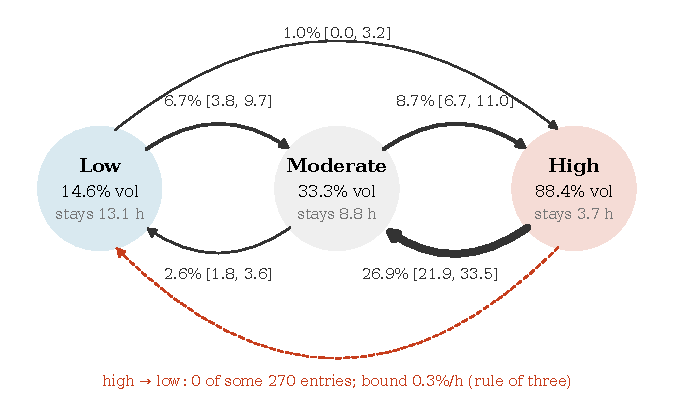
\includegraphics[width=0.88\textwidth]{figures/fig6_transitions.pdf}
  \caption{Transition geometry of the $K{=}3$ return model on the estimation window: hourly transition probabilities with $95\%$ parametric-bootstrap intervals, arrow width increasing with the probability; each node gives the state's annualised volatility and expected duration. The full-sample fit archived only the diagonal of $\hat A$ and the stationary distribution; the off-diagonal probabilities are reconstructed from them with the original fit's boundary estimate $\hat A_{31} = 0$ imposed, so the zero is an input here, and the sub-period fit (Figure~\ref{fig:dist}b) estimates it independently. The bound on $\hat A_{31}$ is the rule of three over the roughly $1{,}000$ high-state hours that the stationary mass implies (Section~\ref{par:funnel}).}
  \label{fig:transitions}
\end{figure}

\subsection{Robustness to Extreme Observations}\label{ssec:robust}

Large prints on a leveraged perpetual --- liquidation cascades, oracle dislocations, thin-book wicks --- are genuine features of the market, so we do not winsorise the estimation sample; the question is whether the high-volatility state rests on a handful of them. It does not. On the hourly sub-period, 3 December 2025 to 28 April 2026 ($T{=}3{,}507$), clipping the extreme $0.1\%$ of returns, four observations, lowers the standard deviation from $50.59$ to $50.30$ bps/h and the refitted high state from $87.7\%$ to $85.4\%$ annualised (Table~\ref{tab:robust}).

The sub-period fit recovers the structure, $12.9\%$, $31.0\%$ and $87.7\%$ against $14.6\%$, $33.3\%$ and $88.4\%$. The high states agree both ways --- $87.7\%$ lies inside the full sample's $[83.0, 94.0]$ and $88.4\%$ inside the sub-period's $[82.1, 93.7]$ --- while the lower two differ by $0.5$ to $0.8$ points beyond each other's intervals; $\hat A_{31} = 0$ again, and exits from the high state again route through the moderate one, with probability $0.26$. Two-hourly candles cover the whole window ($2{,}500$ bars, annualised with $\sqrt{12\cdot 365}$) and give $11.0\%$, $31.6\%$ and $88.8\%$, with a high-state mass of $21.0\%$ against $20.0\%$. Only the boundary result weakens, to $\hat A_{31} \approx 0.01$, as it must when a two-hour bar can contain a passage through the moderate state; it stays an hourly statement.

\paragraph{More than three states.} On the sub-period, with 40 starts each and both larger models converging, BIC is $-28{,}356.8$ for $K{=}2$, $-28{,}533.4$ for $K{=}3$, $-28{,}557.0$ for $K{=}4$ and $-28{,}482.2$ for $K{=}5$, so $K{=}4$ wins, by $23.6$ points; the $K{=}2$ and $K{=}3$ figures reproduce the archived sub-sample fit to the second decimal. We keep $K{=}3$ although $K{=}4$ is estimable. The gain is small beside the $176.6$ points $K{=}3$ adds to $K{=}2$; $K{=}5$ adds only $7.5$ log-likelihood points to $K{=}4$, a pattern a finer discretisation of one heavy-tailed distribution would also produce; the $K{=}4$ volatilities, $11.1$, $24.8$, $55.8$ and $134.9$ bps/h, form a near-geometric ladder with ratios of $2.2$ to $2.4$ whose top rung sits where a Gaussian mixture must place mass to reach the tails; and a Student-$t$ GARCH beats the three-state model on BIC with five parameters (Section~\ref{ssec:diagnostics}). The binding constraint is the Gaussian emission, not the number of volatility levels, and more than three states in one asset have little ex-ante economic interpretation \citep{ang2012}.

\subsection{Inference}\label{ssec:inference}

The standard errors of Table~\ref{tab:regime-params} come from a parametric bootstrap: $500$ series simulated from the fitted chain, state paths started at $\hat\pi^\infty$, each refitted with $K{=}3$ from the generating parameters; against full multi-start refits on 25 paired replications this shortcut costs $0.055$ nats on average and moves $\hat\sigma$ by $0.014$ bps/h. Volatilities and transitions are precise, every $\hat\sigma_k$ having a coefficient of variation below $3.5\%$; the drifts are not.

\subsection{Residual Diagnostics and Benchmarks}\label{ssec:diagnostics}

Conditional independence given the state is testable, and worth testing, since GARCH-type clustering is the competing explanation for a three-state fit. We standardise returns by the one-step predictive moments \eqref{eq:cond-mean}--\eqref{eq:cond-var} from the \emph{filtered} posterior; the smoothed posterior conditions on $r_t$ itself and gives spurious results --- $Q(z^2)(10) = 53.3$, $p < 10^{-7}$, with near-Gaussian residuals --- shown in Table~\ref{tab:diagnostics} for contrast. Raw returns on the sub-period cluster overwhelmingly, $Q(z^2)(10) = 470.7$ and $Q(|z|)(10) = 976.0$, both $p < 10^{-90}$. The chain absorbs most of it --- $Q(z^2)(10)$ falls to $2.4$ and ARCH-LM from $270.3$ to $2.4$ --- but not all: $Q(z^2)$ has little power against ARCH when residuals are as leptokurtic as these, and the tail-robust $Q(|z|)(24) = 96.0$ still rejects. The chain also leaves heavier tails than it started with, an excess kurtosis of $14.4$ against $6.9$. The \MSAR\ residuals fail outright ($Q(10) = 42.6$, excess kurtosis $78.9$).

Against benchmarks outside its family (Table~\ref{tab:benchmarks}) the three-state \HMM\ beats a single Gaussian and a Gaussian GARCH(1,1) by $1{,}422$ and $831$ BIC points but not a Student-$t$ GARCH(1,1), which wins on BIC ($-28{,}583$ against $-28{,}533$) with five parameters against fourteen while losing on AIC ($-28{,}614$ against $-28{,}620$). That winner is near-integrated, $\hat\alpha + \hat\beta = 0.99998$ against the bound of $0.99999$ imposed in estimation, so its unconditional variance is barely finite, and with $\hat\nu = 3.35$ its innovations have no finite kurtosis: it buys likelihood with tails. Both results point to a Student-$t$ or generalised-hyperbolic emission \citep{foroni2024hidden}, and the case for the regime model rests on what GARCH does not deliver: a state decomposition, a transition geometry and a state-conditional object that aligns with the funding model.

\subsection{Goodness of Fit and Posteriors}

Figure~\ref{fig:dist}(a) overlays the stationary mixture $\sum_k \pi_k^\infty\, \varphi(r;\hat\mu_k,\hat\sigma_k^2)$ on the sub-period histogram: the mixture tracks the body, and the high state carries almost all the mass beyond $\pm 3\hat\sigma_2$, about $\pm 100$ bps/h. Figure~\ref{fig:dashboard} follows the posteriors through time. The February 2026 decline to \$62{,}883 coincides with concentrated high-volatility mass, a move of funding off its floor and a shift of the funding posterior, but high-volatility hours recur throughout the window, as the durations imply. The state-implied volatility $\hat\sigma_t^{\text{cond}} = (\sum_k \Prob(S_t=k\given\Filt_t)\,\hat\sigma_k^2)^{1/2}$, averaged over the trailing 24 hours as realised volatility is, tracks it closely; we have not analysed the lead--lag structure between the two.

\begin{figure}[!htbp]
  \centering
  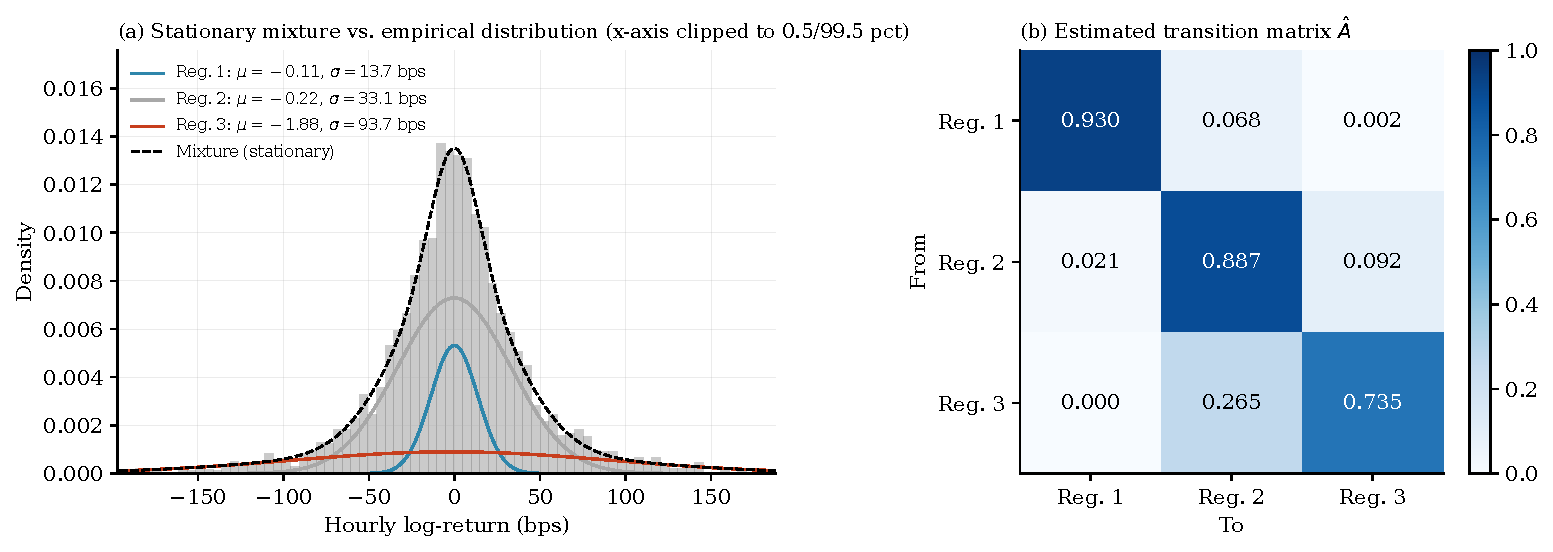
\includegraphics[width=\textwidth]{figures/fig2_distributions.pdf}
  \caption{$K{=}3$ Gaussian \HMM\ on hourly log-returns, fitted to the hourly sub-period (3 Dec 2025 -- 28 Apr 2026, $T = 3{,}507$), the window on which hourly returns survive. \textbf{(a)} Empirical density (grey) against the stationary mixture, components weighted by $\pi^\infty$; the horizontal range is truncated at the $0.5$th and $99.5$th percentiles, so the panel speaks for the body of the distribution, not its tails. \textbf{(b)} Estimated kernel $\hat A$; the zero at $(3,1)$ is the high-to-low transition of Section~\ref{par:funnel}. Reg.~$k$ is State~$k$ of Table~\ref{tab:regime-params}.}
  \label{fig:dist}
\end{figure}

\begin{figure}[!htbp]
  \centering
  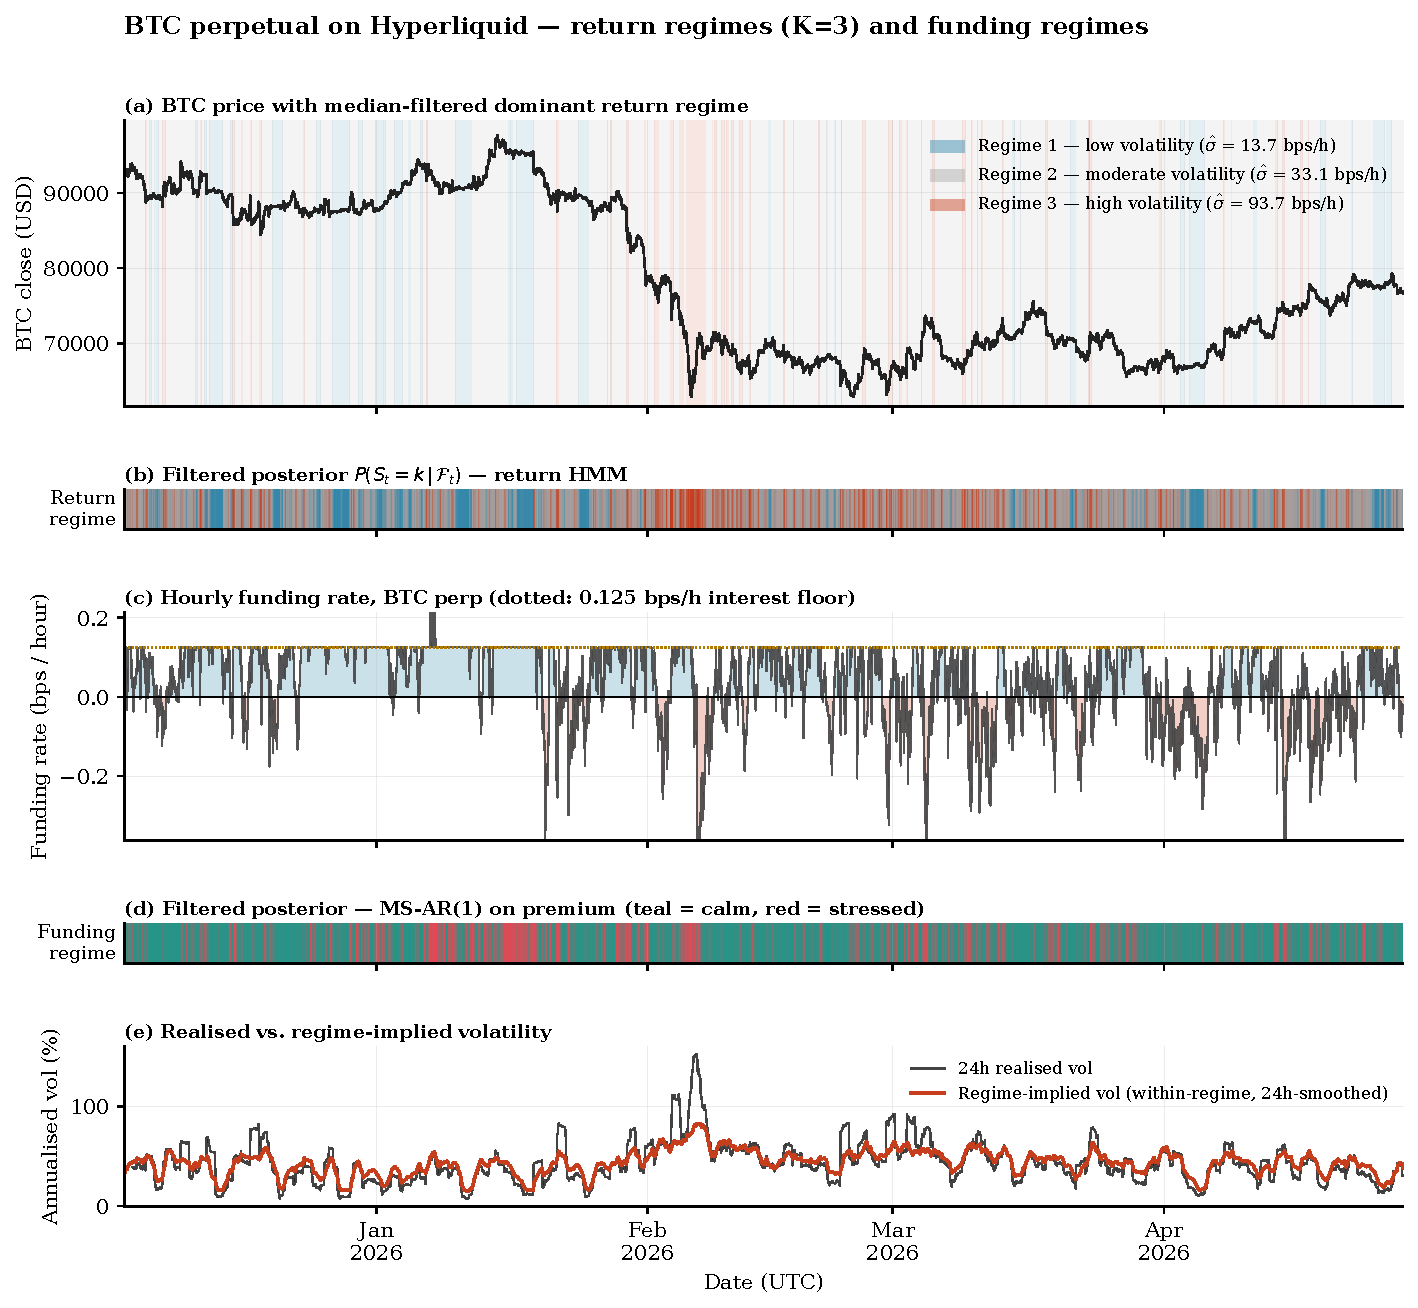
\includegraphics[width=\textwidth]{figures/fig1_regime_dashboard.pdf}
  \caption{State-detection dashboard over the hourly sub-period, 3 Dec 2025 -- 28 Apr 2026 ($T = 3{,}507$). \textbf{(a)} Closing price, shaded by the dominant return state after a centred seven-hour median filter, which is non-causal and presentational only; panel (b) is the causal object. \textbf{(b)} Filtered posterior $\Prob(S_t = k\given\Filt_t)$ of the $K{=}3$ \HMM\ as mixed colour, blue, grey and red for the low-, moderate- and high-volatility states. \textbf{(c)} Hourly funding rate; the horizontal segments at $0.125$ bps/h are the floor of Section~\ref{ssec:clamp}, and the vertical range runs from the $0.5$th to the $99.5$th percentile with a margin and headroom above the floor, so a few extreme prints fall outside it. \textbf{(d)} Filtered posterior of the \MSAR\ on the premium re-estimated on this window, where the half-life ordering is reversed (Section~\ref{ssec:msar-robust}); it is not the fit of Table~\ref{tab:funding-params}. \textbf{(e)} 24-hour realised volatility against the 24-hour trailing mean of the state-implied conditional volatility, both annualised; the latter is a nowcast, not a forecast.}
  \label{fig:dashboard}
\end{figure}

% =========================================================================
\section{Regime Estimation: Funding Premium}\label{sec:funding}

\subsection{Estimated Parameters}

Table~\ref{tab:funding-params} reports the \MSAR(1) on the paper-window premium. The calm regime has $\hat\sigma_1 = 0.53$ bps and $\hat\phi_1 = 0.981$; the stressed regime has $\hat\sigma_2 = 2.68$ bps, $5.1$ times larger, and $\hat\phi_2 = 0.804$. The levels, $\hat\mu_1 = -2.78$ and $\hat\mu_2 = -3.22$ bps, sit beside the sample mean: the regimes differ in volatility and persistence, not in level. Near the unit root the half-life is steep in $\phi$ --- $\mathrm{d}\tau/\mathrm{d}\phi \approx 1{,}860$ hours per unit at $0.981$ --- so even with a standard error of $0.0037$ the calm half-life is known only to within a factor of two, $22$ to $49$ hours. $\hat\phi_1$ still separates from unity: its $t$-ratio of $-5.3$ clears the Dickey--Fuller $1\%$ value of about $-3.4$ that a test on the stationarity boundary faces.

\begin{table}[!htbp]
  \centering
  \caption{\MSAR(1) parameter estimates for the funding premium $y_t$ (8h-equivalent bps). $\hat\mu_k$ is the regime \emph{level} in \eqref{eq:msar}, not an intercept; half-life follows~\eqref{eq:halflife}. Parenthesised figures are standard errors of $\hat\phi_k$, and the intervals are delta-method; Section~\ref{sec:limitations} explains why both are indicative rather than exact.}
  \label{tab:funding-params}
  % Manuscript copy. Window: 2 Oct 2025 -- 28 Apr 2026 (T_eff = 5,000), NOT the
% shipped sub-sample. Source of every number:
%   output/diagnostics.json -> tests[] -> msar block whose window is
%   "paper window 2 Oct 2025 - 28 Apr 2026 (T=5,001)".
% The numbers come from `make diagnostics` (output/diagnostics.json); this file
% is maintained by hand, and tests/test_paper_window_msar.py pins the agreement.
% Do NOT overwrite it with output/tables/table3_funding_params.tex, which is the
% sub-sample fit under the same name.
\begin{tabular}{lrrrrr}
\toprule
Regime & $\hat\mu_k$ (bps) & $\hat\phi_k$ & $\hat\sigma_k$ (bps) & Half-life (h) & 95\% CI \\
\midrule
1 (calm)     & $-2.78$ & 0.9807 & 0.525 & 35.6 & $[22.2,\ 48.9]$ \\
             &         & (0.0037) &     &      &                 \\
2 (stressed) & $-3.22$ & 0.8040 & 2.681 & 3.2  & $[1.5,\ 4.8]$   \\
             &         & (0.0462) &     &      &                 \\
\midrule
\multicolumn{6}{l}{\footnotesize Ratio $\hat\tau_1/\hat\tau_2 = 11.2$ (s.e.\ 4.2; 95\% CI $[3.0,\ 19.4]$, delta method on the full covariance)} \\
\multicolumn{6}{l}{\footnotesize $\log\mathcal{L} = -4808.53$, AIC $= 9633.1$, BIC $= 9685.2$, $T_{\text{eff}} = 5{,}000$} \\
\bottomrule
\end{tabular}

\end{table}

\subsection{The Mean-Reversion Asymmetry}

The half-lives are about $36$ hours calm and $3.2$ hours under stress, a ratio of $11.2$ with a delta-method $95\%$ interval of $[3.0, 19.4]$ (Figure~\ref{fig:funding}): on this window the premium reverts an order of magnitude faster under stress. A size-of-prize mechanism would give this sign. A calm dislocation of a few basis points may not cover the fees, margin and inventory risk of the offsetting basis trade, so capital is not deployed and the dislocation decays slowly; a stressed one makes funding a first-order part of position PnL, clears those costs and is arbitraged back within hours. The argument concerns the size of the mispricing, not liquidity, which on its own would predict the opposite ordering. The specification is a state-dependent Ornstein--Uhlenbeck process. We know of no comparable estimate for a decentralised perpetual, but ours is a single-venue, single-asset point estimate and we claim no priority on its magnitude. Section~\ref{ssec:msar-robust} shows that the ordering belongs to one episode.

\begin{figure}[!htbp]
  \centering
  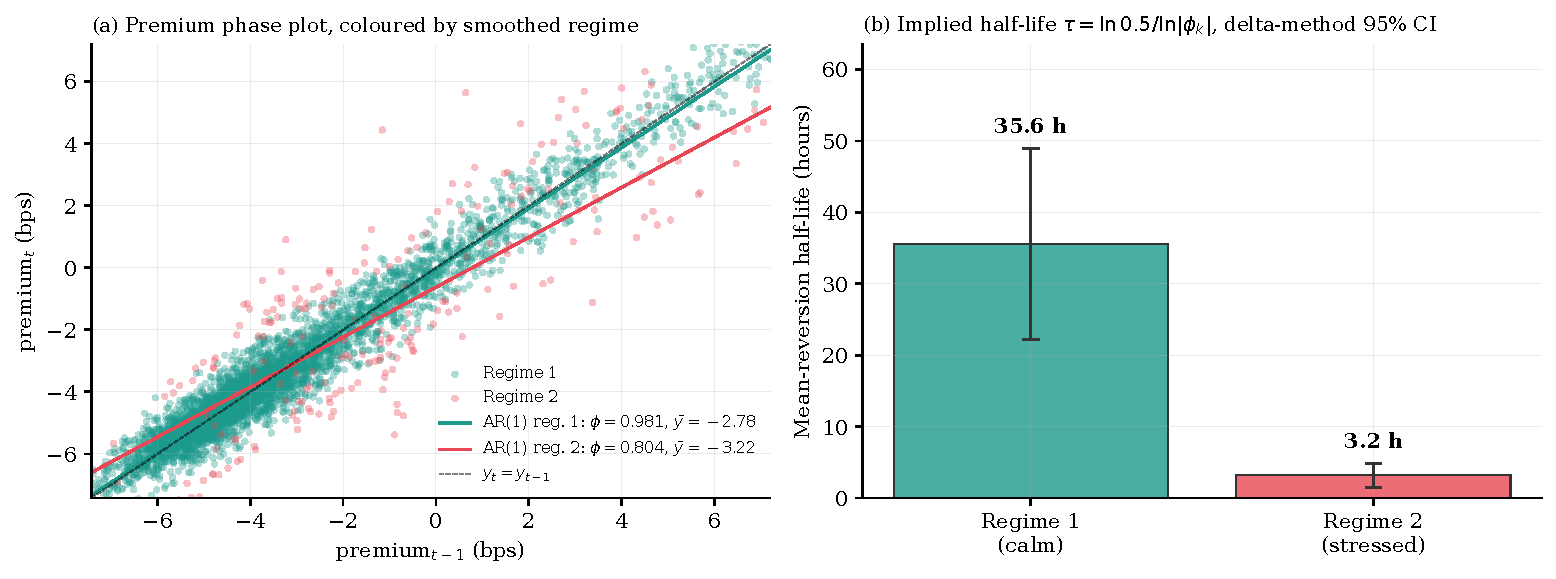
\includegraphics[width=\textwidth]{figures/fig3_funding_dynamics.pdf}
  \caption{Funding-premium dynamics under the \MSAR(1) of Table~\ref{tab:funding-params}. \textbf{(a)} Phase plot of $(y_{t-1}, y_t)$ in bps, coloured by the modal \emph{smoothed} regime, an in-sample diagnostic only; the lines are the regime-conditional fits $\hat\mu_k(1-\hat\phi_k) + \hat\phi_k y_{t-1}$. Both axes are truncated at the $0.5$th and $99.5$th percentiles, so the October 2025 excursion to $+23.61$ bps that identifies the stressed state falls outside the range. \textbf{(b)} Half-life per regime with delta-method intervals.}
  \label{fig:funding}
\end{figure}

\subsection{Specification Robustness and the Precision of the Asymmetry}\label{ssec:msar-robust}

\paragraph{Two optima, and the frequent one is wrong.} The likelihood of \eqref{eq:msar} has two well-separated maxima on this series, and each of our $240$ estimations reaches one of them (Figure~\ref{fig:optima}). The inferior one lies $20.1$ points lower, a likelihood ratio of order $10^{8}$, yet attracts most estimations: $24$ of the paper's $40$, and across six disjoint blocks of $40$ seeds the inferior mode attracts between $20$ and $30$ of the $40$ estimations, while the ranking of the two modes never changes. It differs from the maximum by $0.13$ in $\hat\phi_2$ ($0.672$ against $0.804$) and $0.003$ in $\hat\phi_1$, which the steep half-life turns into a ratio of $24.6$ instead of the $11.2$ of Table~\ref{tab:funding-params}. \texttt{statsmodels} runs no random-start search unless asked, and even with a $40$-draw search a single estimation lands on the inferior optimum three times in five: a Markov-switching result resting on a nonlinear function of $\hat\phi$ needs a recorded multi-start protocol and a reported terminal log-likelihood. We set $K{=}2$ on interpretability and on the small number of stress episodes the window contains.

\begin{figure}[!htbp]
  \centering
  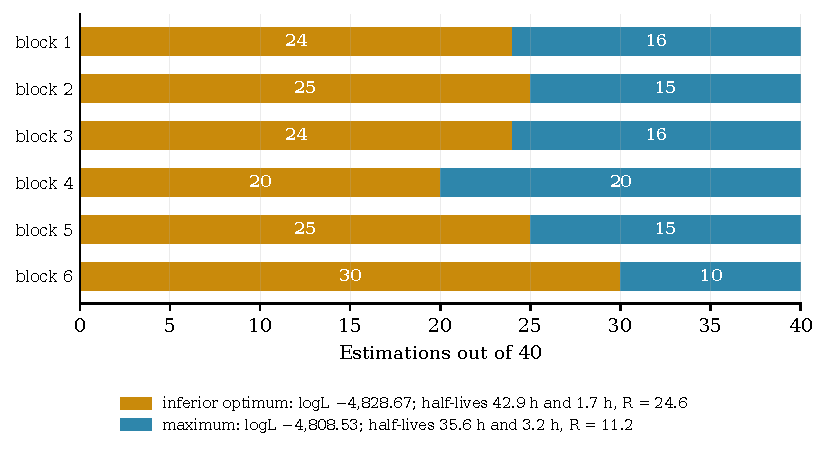
\includegraphics[width=0.74\textwidth]{figures/fig9_optima.pdf}
  \caption{The two optima of the premium likelihood on the paper window. Each bar is a block of $40$ consecutive seeds (the first starts at seed $20260802$), split by the optimum each estimation reaches; the legend gives what each optimum implies.}
  \label{fig:optima}
\end{figure}

\paragraph{Where the asymmetry lives.} The premium series can be refitted on any window (Figure~\ref{fig:october}b). On the 3 December 2025 -- 28 April 2026 sub-period the ordering reverses, $7.1$ hours calm against $24.8$ stressed, at $0.29$ with a $95\%$ interval of $[0.05, 0.52]$; $36$ of $40$ estimations reach that optimum, the other four fail to converge, and none finds a better one. On the whole series, 2 October 2025 to 30 September 2026 ($T = 8{,}737$), the original ordering returns at $4.55$, $[1.95, 7.15]$. The sub-period contains the February 2026 episode entire, including the premium minimum of $-10.55$ bps on 6 February; it lacks the maximum, $+23.61$ bps in one hour of the 10 October 2025 crash (Figure~\ref{fig:october}a), inside the two-hour bar that sets the $1{,}498$ bps bound of Table~\ref{tab:summary}. The stressed state is identified by that hour, not by the February selloff: a window excluding October does not identify the state, and one diluting it attenuates the estimate. Nor do $[3.0, 19.4]$ and $[1.95, 7.15]$ bracket the ratio: the window from the end of the estimation sample to 30 September 2026 gives an interval ending at $0.49$, disjoint from both and on the far side of unity.

Fourteen overlapping windows of $2{,}500$ hours, stepped $450$, localise the effect (Figure~\ref{fig:rolling}, Table~\ref{tab:rolling}). Only the first, the one containing 10 October 2025, places its interval above unity, at $39.17$ with $[7.6, 70.8]$; two others have point estimates above one, $2.94$ and $1.11$, without separating from it, and eleven of the fourteen fall below one outright and nine of those exclude unity. The estimate falls as October leaves the window, crosses unity at the turn of the year and never returns, while the mean drawdown deepens from $21$ to $47$ per cent: one episode, then a baseline. Overlapping by $82\%$, they are fourteen views of a series holding three disjoint windows of this length, not fourteen tests, and twelve months with one drawdown support no cyclical reading.

\paragraph{One observation carries the significance.} The 10 October hour is a genuine observation, not a recording error, and it stays in every main estimate, Table~\ref{tab:funding-params} included. We replace it only to measure what it carries: a two-state model can devote its high-variance state to a single extreme hour, and this one is two and a half times the next largest. Replacing it with that next largest value, $9.52$ bps, moves the paper-window ratio from $11.19$ to $3.04$ and deleting it to $1.83$, both on intervals that cover unity, because $\hat\tau_{\text{stressed}}$ moves from $3.18$ hours to $11.15$ and $18.12$ while the calm half-life barely shifts (Figure~\ref{fig:october}b, Table~\ref{tab:sensitivity}). Winsorising the upper $1$ per cent, fifty hours, still leaves $4.49$ with an interval above unity: the tail carries part of the effect, but the exclusion of unity rests on one hour in $5{,}001$.

The converse is the sharper test. On the window from the end of the estimation sample to 30 September 2026 the ratio is $0.226$, $11.0$ hours calm against $48.7$ stressed, its $95\%$ interval ending at $0.49$ with the lower end left open by the delta method: there the stressed state is the persistent one. Overwriting a single hour with a synthetic $+23.61$ bps, at each quartile of that window in turn, raises it to $18.0$, $11.4$ and $4.3$ --- a factor of $19$ to $79$ on one observation in $3{,}736$. At the first point the manufactured ratio is even significant, $[1.97, 33.98]$; the other two delta-method intervals cover unity. We report these as fragility, not as estimates: one hour can manufacture an asymmetry of the headline's order, significance included, and where it falls decides how large.

\begin{figure}[!htbp]
  \centering
  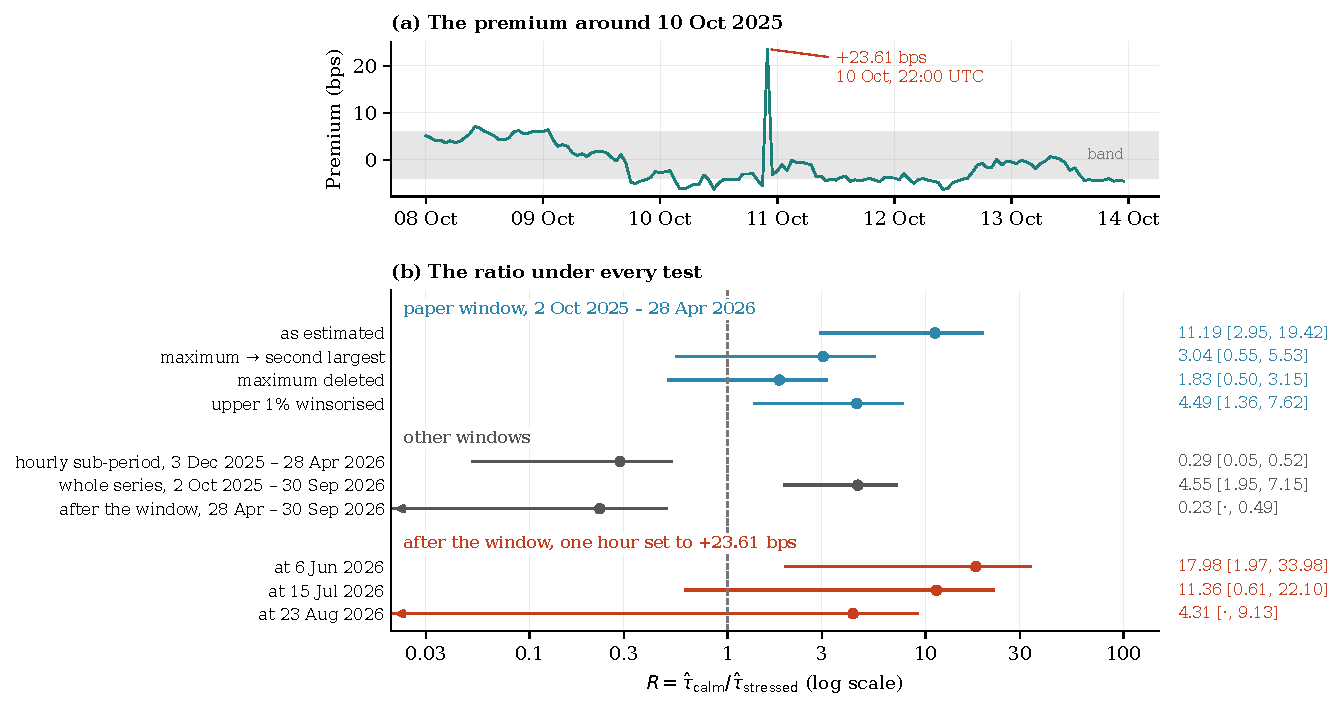
\includegraphics[width=\textwidth]{figures/fig7_october_hour.pdf}
  \caption{The hour that carries the asymmetry. \textbf{(a)} Hourly premium, 8--13 October 2025, against the band; the hour of 10 October 22:00 UTC is the maximum of the whole series. \textbf{(b)} The half-life ratio with its $95\%$ delta-method interval on the paper window and its upper-tail variants (Table~\ref{tab:sensitivity}), on the other windows, and on the later window with one hour overwritten at each quartile; a lower end the delta method returns negative is left open (arrow).}
  \label{fig:october}
\end{figure}

\begin{figure}[!htbp]
  \centering
  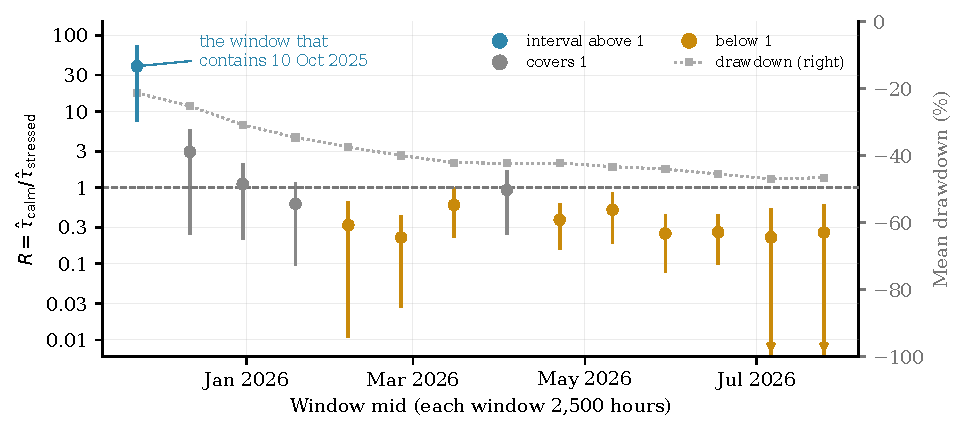
\includegraphics[width=\textwidth]{figures/fig8_rolling.pdf}
  \caption{Rolling estimates of the half-life ratio, windows of $2{,}500$ hours stepped by $450$, at their mid-points: blue if the $95\%$ interval lies above unity, grey if it covers unity, ochre if it lies below; arrows mark lower ends the delta method leaves open. The dotted line with squares is the mean drawdown from the running price peak (right axis). Table~\ref{tab:rolling} lists the estimates.}
  \label{fig:rolling}
\end{figure}

\paragraph{What the later data replicate, and what we claim.} Over the $3{,}736$ hours after the estimation window, $51.7\%$ of funding observations sit exactly on the interest floor, against $46.0\%$ inside it: the censoring persists, if anything more often. The premium's two-state structure does not: the ratio of conditional standard deviations across states falls from $5.1$ to $2.1$, the reversed half-life ordering seen through the variance rather than the persistence. The asymmetry is therefore a property of the October 2025 episode, not a parameter of the Hyperliquid BTC funding premium. Table~\ref{tab:funding-params} describes that episode, and the size-of-prize mechanism remains a candidate explanation for it, which only several such episodes could establish.

% =========================================================================
\section{Implications}\label{sec:trading}

Neither implication is tested (Section~\ref{sec:limitations}). \emph{Position sizing.} The filtered posterior in \eqref{eq:cond-mean}--\eqref{eq:cond-var} gives a one-step conditional variance that a mean-variance rule $w_t = \E[r_{t+1}\given\Filt_t]/(\lambda \Var(r_{t+1}\given\Filt_t))$ would turn into time-varying positions without a separate volatility target. Its within-state term spans $14.6\%$ to $88.4\%$ annualised, a $6.1$-fold range; its between-state term never exceeds $0.3\%$ of the forecast variance, the state means spanning only $6.1$ bps/h, so regime uncertainty as such does not move positions for this asset, though it would for one with a larger spread of state-conditional drifts. \emph{Funding-aware execution.} Calm-regime funding is a slow carry cost and stressed-regime funding a transient, but the only available figure rests on $\hat\tau_{\text{stressed}} = 3.2$ hours, which becomes $11.15$ or $18.12$ hours if one observation changes (Table~\ref{tab:sensitivity}) and is $49$ hours on the window after April 2026 (Section~\ref{ssec:msar-robust}). Whether an execution schedule could exploit the October pattern is a backtest's question, and we do not answer it.

% =========================================================================
\section{Limitations}\label{sec:limitations}

\emph{Scope.} Every result is in-sample and descriptive. Posteriors are evaluated at the full-sample estimate, the filtered/smoothed distinction is a property of the recursions rather than a real-time claim, and no walk-forward, backtest or transaction-cost exercise is run.

\emph{External validity.} One asset on one venue: seven months of returns with a single macro drawdown and twelve months of premium containing a single funding episode, compared with two exchanges in one market phase, in which their premiums sat below the band; with persistently positive premia the ordering could change. We would not carry the parameter values to other assets, venues or periods.

\emph{Inference.} The \HMM\ bootstrap conditions on the Gaussian emission, which the diagnostics reject; a block bootstrap would relax that, and the heteroskedasticity left after the state decomposition makes a Markov-switching GARCH \citep{haas2004new,ardia2019} the natural next model. The \MSAR\ standard errors come from the Hessian of a Gaussian likelihood its residuals reject badly --- excess kurtosis of $79$, a Jarque--Bera statistic more than forty times the \HMM's --- so its delta-method intervals are indicative; a sandwich or block-bootstrap covariance would be the repair, and we have not computed one. The ordering of the two point estimates, $35.6$ hours against $3.2$, does not involve the covariance, but $\hat\phi_{\text{stressed}}$ is itself set by one observation.

\emph{Specification.} The three-state \HMM\ does not dominate a Student-$t$ GARCH(1,1) on BIC, and we run no encompassing test. No third premium state is tested, the nuisance-parameter problem of Section~\ref{ssec:hmm} applying here too \citep{davies1987,hansen1992}. The premium index is a within-hour average, which induces a moving-average component, so the AR(1) is misspecified and $\hat\phi$ biased; a Markov-switching ARMA(1,1) is the next step.

\emph{Replication.} Every funding-side result reproduces from source; the hourly return panel's first two months do not (Data and Code Availability).

% =========================================================================
\section{Conclusion}\label{sec:conclusion}

The measurement we would most like carried forward is the censoring. One rule, common to the major perpetual venues, pins funding to the interest rate in $46\%$ of Hyperliquid's settlements and in only $6$ to $8\%$ of Binance's and Bybit's over the same window, because the exchanges' premiums sit just below the band while Hyperliquid's straddles its edge. Work on Hyperliquid funding should model the premium, and cross-venue comparisons that read funding as positioning should compare premiums, with their windows and indices in view. Why the premiums sit where they do --- index construction, the depth of arbitrage capital, the mix of traders --- is the question the measurement opens, and it needs more venues, assets and market phases.

On returns, the estimated probability that hourly volatility moves directly from the high state to the low is zero, with a $95\%$ bound of $0.3\%$ per hour. On the premium, the asymmetry in mean reversion describes the October 2025 episode and not the series. The natural extensions are a Student-$t$ or generalised-hyperbolic emission \citep{foroni2024hidden}, time-varying transition probabilities driven by covariates such as open interest or liquidity \citep{filardo1994business}, and a regime-conditional carry backtest once the asymmetry has been seen across several episodes.

% =========================================================================
\section*{Data and Code Availability}
\addcontentsline{toc}{section}{Data and Code Availability}

\begin{sloppypar}
The estimation panel comes from Hyperliquid's public REST API --- \texttt{candleSnapshot} (hourly OHLCV candles of traded prices) and \texttt{fundingHistory} (hourly funding rate and premium index) --- retrieved on 28 April 2026; the premium series beyond it and the two-hourly candles were retrieved from the same endpoints in August and October 2026. Binance and Bybit data come from their public endpoints (Binance: \texttt{fapi/v1/fundingRate} and \texttt{fapi/v1/premiumIndexKlines}; Bybit: \texttt{v5/market/funding/history} and \texttt{v5/market/premium-index-price-kline}), retrieved on 6 October 2026. All endpoints are unauthenticated, and no proprietary or licensed data are used.
\end{sloppypar}

The \emph{funding and premium} series is fully replicable: \texttt{fundingHistory} has no retention limit, and an independent re-retrieval agreed with the archived panel to machine precision on all $3{,}507$ overlapping hours. The hourly \emph{price} series is not: the results that use hourly prices before 3 December 2025 --- the log-return and closing-price rows of Table~\ref{tab:summary}, Tables~\ref{tab:modelsel}--\ref{tab:regime-params}, Figure~\ref{fig:transitions}, which draws the full-sample kernel, and the price labels of Figure~\ref{fig:windows} --- rest on the original extract. Every other figure is drawn from the shipped data and artifacts: Figures~\ref{fig:dist} and~\ref{fig:dashboard} on the archived hourly panel of 3 December 2025 -- 28 April 2026, and Figure~\ref{fig:funding} on the paper window of the premium series. The materials also contain two-hourly candles for the whole span (Figure~\ref{fig:windows}); the exchange's two-hourly window will cease to cover 2 October 2025 in late November 2026, its four-hourly window in 2028.

Code, data, the fitted parameters behind every table, figure and quoted fit in machine-readable form --- except the full-sample $K{=}2$ fit, whose log-likelihood survives only in Table~\ref{tab:modelsel} --- and the seeds and multi-start protocol behind each estimate are in the replication repository,
\begin{center}\url{https://github.com/gelatotrade/HMM-Decentralised-Perpetual-Futures}.\end{center}

\section*{Competing Interests}
\addcontentsline{toc}{section}{Competing Interests}

The author does not trade on Hyperliquid, Binance or Bybit, holds no equity, advisory or employment relationship with any of them, and received no compensation connected with this work; no third party reviewed or influenced the analysis. The Hyperliquid Research Collective, which publishes this research under the author's name alongside this posting, is an independent group despite the shared name and has no relationship to Hyperliquid; the author's work for it is unpaid.

\section*{Funding}
\addcontentsline{toc}{section}{Funding}

This research received no specific grant from any funding agency in the public, commercial or not-for-profit sectors.

% =========================================================================
\clearpage
\bibliographystyle{plainnat}
\begin{thebibliography}{99}\setlength{\itemsep}{1pt}\small\raggedright

\bibitem[Ackerer et~al.(2026)]{ackerer2024}
Ackerer, D., Hugonnier, J., and Jermann, U. (2026).
\newblock Perpetual futures pricing.
\newblock \textit{Mathematical Finance} 36(3), 481--499.
\newblock \url{https://doi.org/10.1111/mafi.70018}.

\bibitem[Alexander et~al.(2020)]{alexander2020bitmex}
Alexander, C., Choi, J., Park, H., and Sohn, S. (2020).
\newblock BitMEX bitcoin derivatives: Price discovery, informational efficiency, and hedging effectiveness.
\newblock \textit{Journal of Futures Markets} 40(1), 23--43.
\newblock \url{https://doi.org/10.1002/fut.22050}.

\bibitem[Ang and Timmermann(2012)]{ang2012}
Ang, A. and Timmermann, A. (2012).
\newblock Regime changes and financial markets.
\newblock \textit{Annual Review of Financial Economics} 4, 313--337.
\newblock \url{https://doi.org/10.1146/annurev-financial-110311-101808}.

\bibitem[Ardia et~al.(2019)]{ardia2019}
Ardia, D., Bluteau, K., and R\"uede, M. (2019).
\newblock Regime changes in Bitcoin GARCH volatility dynamics.
\newblock \textit{Finance Research Letters} 29, 266--271.
\newblock \url{https://doi.org/10.1016/j.frl.2018.08.009}.

\bibitem[Binance(2026)]{binance_funding_docs}
Binance (2026).
\newblock Introduction to Binance Futures funding rates. Binance Support. Accessed 6 October 2026.
\newblock \url{https://www.binance.com/en/support/faq/introduction-to-binance-futures-funding-rates-360033525031}.

\bibitem[Bybit(2026)]{bybit_funding_docs}
Bybit (2026).
\newblock Introduction to funding rate. Bybit Help Center. Accessed 6 October 2026.
\newblock \url{https://www.bybit.com/en/help-center/article/Introduction-to-Funding-Rate}.

\bibitem[Cho and White(2007)]{cho2007}
Cho, J.~S. and White, H. (2007).
\newblock Testing for regime switching.
\newblock \textit{Econometrica} 75(6), 1671--1720.
\newblock \url{https://doi.org/10.1111/j.1468-0262.2007.00809.x}.

\bibitem[Cont(2007)]{cont2005volatility}
Cont, R. (2007).
\newblock Volatility clustering in financial markets: Empirical facts and agent-based models.
\newblock In G.~Teyssi\`ere and A.~P. Kirman (eds.), \textit{Long Memory in Economics},
  Springer, Berlin, pp.~289--309.
\newblock \url{https://doi.org/10.1007/978-3-540-34625-8_10}.

\bibitem[Davies(1987)]{davies1987}
Davies, R.~B. (1987).
\newblock Hypothesis testing when a nuisance parameter is present only under the alternative.
\newblock \textit{Biometrika} 74(1), 33--43.
\newblock \url{https://doi.org/10.1093/biomet/74.1.33}.

\bibitem[Filardo(1994)]{filardo1994business}
Filardo, A.~J. (1994).
\newblock Business-cycle phases and their transitional dynamics.
\newblock \textit{Journal of Business \& Economic Statistics} 12(3), 299--308.
\newblock \url{https://doi.org/10.1080/07350015.1994.10524545}.

\bibitem[Foroni et~al.(2025)]{foroni2024hidden}
Foroni, B., Merlo, L., and Petrella, L. (2025).
\newblock Hidden Markov graphical models with state-dependent generalized hyperbolic distributions.
\newblock \textit{Canadian Journal of Statistics}, article e70030.
\newblock \url{https://doi.org/10.1002/cjs.70030}.

\bibitem[Gassiat and Boucheron(2003)]{gassiat2003}
Gassiat, E. and Boucheron, S. (2003).
\newblock Optimal error exponents in hidden Markov models order estimation.
\newblock \textit{IEEE Transactions on Information Theory} 49(4), 964--980.
\newblock \url{https://doi.org/10.1109/TIT.2003.809574}.

\bibitem[Giudici and Abu~Hashish(2020)]{giudici2020}
Giudici, P. and Abu~Hashish, I. (2020).
\newblock A hidden Markov model to detect regime changes in cryptoasset markets.
\newblock \textit{Quality and Reliability Engineering International} 36(6), 2057--2065.
\newblock \url{https://doi.org/10.1002/qre.2673}.

\bibitem[Haas et~al.(2004)]{haas2004new}
Haas, M., Mittnik, S., and Paolella, M.~S. (2004).
\newblock A new approach to Markov-switching GARCH models.
\newblock \textit{Journal of Financial Econometrics} 2(4), 493--530.
\newblock \url{https://doi.org/10.1093/jjfinec/nbh020}.

\bibitem[Hamilton(1989)]{hamilton1989}
Hamilton, J.~D. (1989).
\newblock A new approach to the economic analysis of nonstationary time series and the business cycle.
\newblock \textit{Econometrica} 57(2), 357--384.
\newblock \url{https://doi.org/10.2307/1912559}.

\bibitem[Hansen(1992)]{hansen1992}
Hansen, B.~E. (1992).
\newblock The likelihood ratio test under nonstandard conditions: testing the Markov switching model of GNP.
\newblock \textit{Journal of Applied Econometrics} 7(S1), S61--S82.
\newblock \url{https://doi.org/10.1002/jae.3950070506}.

\bibitem[He et~al.(2022)]{he2022perp}
He, S., Manela, A., Ross, O., and von Wachter, V. (2022).
\newblock Fundamentals of perpetual futures.
\newblock arXiv:2212.06888.

\bibitem[Hugonnier and Jermann(2025)]{hugonnier2025clamp}
Hugonnier, J. and Jermann, U.~J. (2025).
\newblock Perpetual futures pricing with stochastic rates and clamp.
\newblock Working paper, SSRN 5610430.
\newblock \url{https://doi.org/10.2139/ssrn.5610430}.

\bibitem[Hyperliquid(2026)]{hyperliquid_funding_docs}
Hyperliquid (2026).
\newblock Funding. Hyperliquid Docs. Accessed 18 August 2026.
\newblock \url{https://hyperliquid.gitbook.io/hyperliquid-docs/trading/funding}.

\bibitem[Kass and Raftery(1995)]{kass1995bayes}
Kass, R.~E. and Raftery, A.~E. (1995).
\newblock Bayes factors.
\newblock \textit{Journal of the American Statistical Association} 90(430), 773--795.
\newblock \url{https://doi.org/10.1080/01621459.1995.10476572}.

\bibitem[Keribin(2000)]{keribin2000}
Keribin, C. (2000).
\newblock Consistent estimation of the order of mixture models.
\newblock \textit{Sankhy\=a: The Indian Journal of Statistics, Series A} 62(1), 49--66.

\bibitem[Kim(1994)]{kim1994dynamic}
Kim, C.-J. (1994).
\newblock Dynamic linear models with Markov-switching.
\newblock \textit{Journal of Econometrics} 60(1--2), 1--22.
\newblock \url{https://doi.org/10.1016/0304-4076(94)90036-1}.

\bibitem[Kim and Park(2025)]{kim2025funding}
Kim, J. and Park, H. (2025).
\newblock Designing funding rates for perpetual futures in cryptocurrency markets.
\newblock Working paper, arXiv:2506.08573.
\newblock \url{https://doi.org/10.48550/arXiv.2506.08573}.

\bibitem[Koki et~al.(2022)]{koki2022bitcoin}
Koki, C., Leonardos, S., and Piliouras, G. (2022).
\newblock Exploring the predictability of cryptocurrencies via Bayesian hidden Markov models.
\newblock \textit{Research in International Business and Finance} 59, 101554.
\newblock \url{https://doi.org/10.1016/j.ribaf.2021.101554}.

\bibitem[Koutmos(2018)]{koutmos2018}
Koutmos, D. (2018).
\newblock Bitcoin returns and transaction activity.
\newblock \textit{Economics Letters} 167, 81--85.
\newblock \url{https://doi.org/10.1016/j.econlet.2018.03.021}.

\bibitem[Machimbo et~al.(2025)]{machimbo2025}
Machimbo, E.~W., Cheruiyot, W., Mocheche, G.~M., and Mutegi, J. (2025).
\newblock Applications of hidden Markov models in detecting regime changes in Bitcoin markets.
\newblock \textit{Asian Journal of Probability and Statistics} 27(7), 127--138.
\newblock \url{https://doi.org/10.9734/ajpas/2025/v27i7781}.

\bibitem[Makarov and Schoar(2020)]{makarov2020trading}
Makarov, I. and Schoar, A. (2020).
\newblock Trading and arbitrage in cryptocurrency markets.
\newblock \textit{Journal of Financial Economics} 135(2), 293--319.
\newblock \url{https://doi.org/10.1016/j.jfineco.2019.07.001}.

\bibitem[Rabiner(1989)]{rabiner1989}
Rabiner, L.~R. (1989).
\newblock A tutorial on hidden Markov models and selected applications in speech recognition.
\newblock \textit{Proceedings of the IEEE} 77(2), 257--286.
\newblock \url{https://doi.org/10.1109/5.18626}.

\bibitem[Schmeling et~al.(2026)]{schmeling2025crypto}
Schmeling, M., Schrimpf, A., and Todorov, K. (2026).
\newblock Crypto carry.
\newblock \textit{Management Science}, articles in advance.
\newblock \url{https://doi.org/10.1287/mnsc.2024.05069}.

\bibitem[Stephens(2000)]{stephens2000label}
Stephens, M. (2000).
\newblock Dealing with label switching in mixture models.
\newblock \textit{Journal of the Royal Statistical Society: Series B} 62(4), 795--809.
\newblock \url{https://doi.org/10.1111/1467-9868.00265}.

\bibitem[Werapun et~al.(2026)]{werapun2026funding}
Werapun, W., Karode, T., Suaboot, J., Arpornthip, T., and Sangiamkul, E. (2026).
\newblock Exploring risk and return profiles of funding rate arbitrage on CEX and DEX.
\newblock \textit{Blockchain: Research and Applications} 7(4), 100354.
\newblock \url{https://doi.org/10.1016/j.bcra.2025.100354}.

\bibitem[Zhivkov(2026)]{zhivkov2026funding}
Zhivkov, P. (2026).
\newblock The two-tiered structure of cryptocurrency funding rate markets.
\newblock \textit{Mathematics} 14(2), 346.
\newblock \url{https://doi.org/10.3390/math14020346}.

\bibitem[Zhivkov et~al.(2026)]{zhivkov2026temporal}
Zhivkov, P., Todorov, V., and Georgiev, S. (2026).
\newblock Temporal dynamics of market microstructure in cryptocurrency perpetual futures:
  Econometric evidence from centralized and decentralized exchanges.
\newblock \textit{International Journal of Financial Studies} 14(5), 103.
\newblock \url{https://doi.org/10.3390/ijfs14050103}.

\end{thebibliography}

% =========================================================================
\clearpage
\appendix
\renewcommand{\thetable}{A\arabic{table}}
\setcounter{table}{0}
\section{Additional Tables}\label{app:tables}

\begin{table}[!htbp]
  \centering
  \caption{Robustness of the $K{=}3$ state volatilities to winsorisation, estimated on the reproducible sub-period (3 Dec 2025 -- 28 Apr 2026, $T=3{,}507$). Winsorisation clips the most extreme $0.1\%$ of hourly returns, four observations in total. Under the $\hat\sigma$-ascending labelling of Section~\ref{ssec:hmm} index and state coincide, so column $k$ is State $k$ of Table~\ref{tab:regime-params}. The estimated probability of a direct high-to-low-volatility transition remains zero in both fits, and the stationary masses move by at most $1.2$ percentage points (high-volatility state $21.2\% \to 22.4\%$, low-volatility state $18.3\% \to 17.3\%$).}
  \label{tab:robust}
  % Manuscript copy. Sub-period 3 Dec 2025 -- 28 Apr 2026 (T = 3,507).
% Source: output/robustness.json -> raw / winsorised -> ann_vol_pct.
% Columns follow the sigma-ascending labelling of the paper: index and state
% coincide, so column k is State k of the regime-parameter table
% (table2_regime_params.tex).
\begin{tabular}{lrrr}
\toprule
Annualised $\hat\sigma$ & 1 low & 2 moderate & 3 high \\
\midrule
Raw ($T=3{,}507$)            & 12.9\% & 31.0\% & 87.7\% \\
Winsorised (extreme 0.1\%)   & 12.6\% & 30.4\% & 85.4\% \\
\bottomrule
\end{tabular}

\end{table}

\begin{table}[!htbp]
  \centering
  \caption{Residual diagnostics. Raw-return and \HMM\ rows use the sub-period panel ($T = 3{,}507$); \MSAR\ rows use the paper window ($T = 5{,}001$, leaving $4{,}999$ residuals --- the autoregressive lag costs one observation and the state-pair construction of the one-step forecast another), because that window's premium series survives and its return series does not. For the \HMM\ rows $z_t$ is standardised by the one-step-ahead mixture mean and the full conditional variance of \eqref{eq:cond-var}; headline rows use filtered (causal) state probabilities, smoothed rows are shown for contrast only.}
  \label{tab:diagnostics}
  % Compact rendering of output/tables/table6_diagnostics.tex for the manuscript.
% Regenerate the source with `make diagnostics`; see output/diagnostics.json for
% the full battery including lag 2 and the sub-sample MS-AR rows.
\small
\setlength{\tabcolsep}{4pt}
\begin{tabular}{lrrrr}
\toprule
\multicolumn{5}{l}{\emph{Panel A: Ljung--Box $Q(\ell)$, $p$-value in brackets}} \\[2pt]
Series & $\ell$ & $Q(z)$ & $Q(z^2)$ & $Q(|z|)$ \\
\midrule
Raw log-returns          & 10 & 6.7 [0.76] & 470.7 [$<$0.0001] & 976.0 [$<$0.0001] \\
                         & 24 & 17.0 [0.85] & 671.2 [$<$0.0001] & 1{,}718.1 [$<$0.0001] \\
\addlinespace
\HMM\ $K{=}3$, filtered  & 10 & 7.9 [0.64] & 2.4 [0.99] & 20.6 [0.024] \\
                         & 24 & 18.3 [0.79] & 5.7 [1.00] & 96.0 [$<$0.0001] \\
\addlinespace
\HMM\ $K{=}3$, smoothed  & 10 & 14.2 [0.16] & 53.3 [$<$0.0001] & 32.8 [0.0003] \\
                         & 24 & 28.2 [0.25] & 92.3 [$<$0.0001] & 78.4 [$<$0.0001] \\
\addlinespace
\MSAR(1), paper window   & 1  & 6.7 [0.0096] & 48.9 [$<$0.0001] & 36.8 [$<$0.0001] \\
                         & 10 & 42.6 [$<$0.0001] & 51.5 [$<$0.0001] & 90.3 [$<$0.0001] \\
\midrule
\multicolumn{5}{l}{\emph{Panel B: heteroskedasticity and normality}} \\[2pt]
Series & ARCH-LM(12) & Jarque--Bera & Skew & Exc.\ kurt. \\
\midrule
Raw log-returns          & 270.3 [$<$0.0001] & 7{,}081 [$<$0.0001] & $-0.26$ & 6.94 \\
\HMM\ $K{=}3$, filtered  & 2.4 [0.9985] & 31{,}101 [$<$0.0001] & $-1.02$ & 14.45 \\
\HMM\ $K{=}3$, smoothed  & 46.1 [$<$0.0001] & 13 [0.0017] & $-0.06$ & 0.27 \\
\MSAR(1), paper window   & 51.4 [$<$0.0001] & 1{,}304{,}072 [$<$0.0001] & 2.80 & 78.93 \\
\bottomrule
\end{tabular}

\end{table}

\begin{table}[!htbp]
  \centering
  \caption{Out-of-family comparison on the sub-period panel ($T = 3{,}507$), all rows on the same raw log-return series with $\text{AIC} = 2k - 2\log\mathcal{L}$ and $\text{BIC} = k\log T - 2\log\mathcal{L}$; lower is better. Log-likelihoods are not scale-free, so mixing return units across rows would decide the ranking by itself. The Student-$t$ GARCH row, which wins on BIC, is near-integrated ($\hat\alpha + \hat\beta = 0.99998$, against the bound of $0.99999$ imposed in estimation) with $\hat\nu = 3.35$: a barely finite unconditional variance, no finite kurtosis. Both qualifications are recorded in \texttt{output/benchmarks.json}.}
  \label{tab:benchmarks}
  % Generated by regime_engine.diagnostics -- do not edit by hand.
% All rows fitted on the same T = 3507 hourly log-returns, in raw
% return units. AIC = 2k - 2logL, BIC = k log T - 2logL; lower is better.
\begin{tabular}{lrrrr}
\toprule
Model & $\log\mathcal{L}$ & \# params & AIC & BIC \\
\midrule
GARCH(1,1)-Student-t & 14,312.1 & 5 & $-$28,614.2 & $-$28,583.4 \\
Gaussian HMM, K=3 & 14,323.8 & 14 & $-$28,619.7 & $-$28,533.4 \\
Gaussian HMM, K=2 & 14,207.0 & 7 & $-$28,400.0 & $-$28,356.8 \\
GARCH(1,1)-Normal & 13,867.3 & 4 & $-$27,726.7 & $-$27,702.0 \\
Gaussian i.i.d. & 13,563.8 & 2 & $-$27,123.5 & $-$27,111.2 \\
\bottomrule
\end{tabular}

\end{table}

\begin{table}[!htbp]
  \centering
  \caption{Rolling \MSAR(1) estimates of $R = \hat\tau_{\text{calm}}/\hat\tau_{\text{stressed}}$ on the premium series, windows of $2{,}500$ hours stepped by $450$, forty starts each; the final $387$ hours of the series fill no further window. \emph{Side} records which side of unity the delta-method interval falls on; $\cdot$ marks a lower endpoint the delta method returns negative, which a half-life cannot be. \emph{Price} is the mean two-hourly closing price over the window and \emph{DD} its mean drawdown from the running peak. Regimes are labelled by $\hat\sigma^2_k$ ascending throughout.}
  \label{tab:rolling}
  \small
  % Generated by regime_engine.oos -- do not edit by hand.
% Rolling MS-AR on the premium series: window 2500 h, step 450 h, 40 starts per fit.
% Regimes are labelled by sigma2 ascending, so R = tau_calm / tau_stressed.
\begin{tabular}{lrrrlcrr}
\toprule
Window mid & $\hat\tau_{\text{calm}}$ & $\hat\tau_{\text{str}}$ & $\hat R$ & 95\% CI & side & price & DD \\
\midrule
2025-11-23 & 50.91 & 1.30 & 39.17 & [7.59, 70.75] & $>1$ & 98{,}691 & $-21\%$ \\
2025-12-11 & 37.71 & 12.81 & 2.94 & [0.26, 5.63] & n.s. & 93{,}944 & $-25\%$ \\
2025-12-30 & 18.26 & 16.42 & 1.11 & [0.22, 2.01] & n.s. & 86{,}913 & $-31\%$ \\
2026-01-18 & 10.98 & 17.96 & 0.61 & [0.10, 1.12] & n.s. & 82{,}165 & $-35\%$ \\
2026-02-06 & 7.59 & 23.63 & 0.32 & [0.01, 0.63] & $<1$ & 78{,}522 & $-37\%$ \\
2026-02-24 & 6.18 & 27.93 & 0.22 & [0.03, 0.41] & $<1$ & 75{,}393 & $-40\%$ \\
2026-03-15 & 4.88 & 8.26 & 0.59 & [0.23, 0.95] & $<1$ & 72{,}701 & $-42\%$ \\
2026-04-03 & 5.79 & 6.24 & 0.93 & [0.25, 1.61] & n.s. & 72{,}487 & $-42\%$ \\
2026-04-22 & 3.41 & 9.05 & 0.38 & [0.16, 0.59] & $<1$ & 72{,}581 & $-42\%$ \\
2026-05-10 & 3.92 & 7.64 & 0.51 & [0.19, 0.83] & $<1$ & 71{,}215 & $-43\%$ \\
2026-05-29 & 4.93 & 19.78 & 0.25 & [0.08, 0.42] & $<1$ & 70{,}321 & $-44\%$ \\
2026-06-17 & 4.39 & 16.87 & 0.26 & [0.10, 0.42] & $<1$ & 68{,}481 & $-45\%$ \\
2026-07-06 & 9.36 & 42.04 & 0.22 & [$\cdot$, 0.51] & $<1$ & 66{,}633 & $-47\%$ \\
2026-07-24 & 10.11 & 39.22 & 0.26 & [$\cdot$, 0.58] & $<1$ & 67{,}110 & $-47\%$ \\
\bottomrule
\end{tabular}

\end{table}

\begin{table}[!htbp]
  \centering
  \caption{Sensitivity of the paper-window asymmetry to the upper tail of the premium. Each row refits \eqref{eq:msar} on $2$ October 2025 -- $28$ April 2026 after one change, with the baseline refitted alongside under the same protocol. \emph{Maximum $\to$ 2nd largest} replaces the $+23.61$ bps observation of 10 October 2025 by $9.52$ bps; \emph{Maximum deleted} removes it.}
  \label{tab:sensitivity}
  % Generated by regime_engine.oos -- do not edit by hand.
% Paper window (T = 5,001). Each row refits the MS-AR after one change
% to the upper tail of the premium; the baseline is refitted alongside.
\begin{tabular}{lrrrrlc}
\toprule
Series & $T$ & $\hat\tau_{\text{calm}}$ & $\hat\tau_{\text{str}}$ & $\hat R$ & 95\% CI & side \\
\midrule
Unchanged & 5{,}001 & 35.55 & 3.18 & 11.19 & [2.95, 19.42] & $>1$ \\
Maximum $\to$ 2nd largest & 5{,}001 & 33.90 & 11.15 & 3.04 & [0.55, 5.53] & n.s. \\
Maximum deleted & 5{,}000 & 33.10 & 18.12 & 1.83 & [0.50, 3.15] & n.s. \\
Winsorised, upper 1\% & 5{,}001 & 42.23 & 9.40 & 4.49 & [1.36, 7.62] & $>1$ \\
\bottomrule
\end{tabular}

\end{table}

\clearpage
\section{Estimation Details}\label{app:estimation}
\renewcommand{\theequation}{B\arabic{equation}}
\setcounter{equation}{0}

\paragraph{Recursions.} The filtered posterior is computed through the forward variable $\alpha_t(i) = \Prob(r_{1:t}, S_t=i\given\theta)$,
\begin{equation}\label{eq:forward}
  \alpha_1(i) = \pi_i\, b_i(r_1), \qquad
  \alpha_{t+1}(j) = \Bigl[\textstyle\sum_i \alpha_t(i) A_{ij}\Bigr]\, b_j(r_{t+1}),
\end{equation}
and the smoothed posterior from the forward and backward variables,
\begin{equation}\label{eq:smoothed}
  \gamma_t(i) \;=\; \frac{\alpha_t(i)\,\beta_t(i)}{\textstyle\sum_j \alpha_T(j)},\qquad
  \beta_t(i) = \textstyle\sum_j A_{ij}\, b_j(r_{t+1})\,\beta_{t+1}(j);
\end{equation}
the Viterbi path replaces the marginalisation in~\eqref{eq:forward} with maximisation. Baum--Welch alternates an E-step for $\gamma$ and the pairwise posteriors $\xi_t(i,j) = \Prob(S_t=i,S_{t+1}=j\given\Filt_T,\theta^{(n)})$ with the closed-form M-step
\begin{equation}\label{eq:mstep}
  \hat A_{ij} = \frac{\sum_t \xi_t(i,j)}{\sum_t \gamma_t(i)},\qquad
  \hat\mu_k = \frac{\sum_t \gamma_t(k)\, r_t}{\sum_t \gamma_t(k)},\qquad
  \hat\sigma_k^2 = \frac{\sum_t \gamma_t(k)\,(r_t-\hat\mu_k)^2}{\sum_t \gamma_t(k)}.
\end{equation}
EM finds local maxima, so we run eight random initialisations and keep the highest terminal log-likelihood. At $T \sim 5{,}000$ the recursions underflow in linear space; we run them in log space with the \emph{logsumexp} trick, vectorised across destination states. The implementation is self-contained and validated against simulated ground truth.

\paragraph{Labelling.} Label switching \citep{stephens2000label} requires an ordering rule, and the natural one for returns, $\hat\mu_1 \le \dots \le \hat\mu_K$, fails here: two of the three means lie within $0.27$ bps/h of each other, well inside their sampling variability. In the parametric bootstrap of Section~\ref{ssec:inference} the $\mu$- and $\sigma$-ascending orderings disagree in $40.2\%$ of replications, and under $\mu$-ascending the $95\%$ interval for the state with $\hat\sigma = 15.6$ bps/h is $[14.6, 90.7]$, against $[14.5, 16.5]$ under $\sigma$-ascending: the first interval measures the sorting rule, not the estimator. A $\mu$-ascending rule would also permute the upper two indices of the full-sample and sub-period fits relative to each other, so that the transition regularity of Section~\ref{par:funnel} would seem not to replicate. The volatilities are separated by many standard errors, and the $\sigma$-ascending order is stable in every fit we report.

\paragraph{The premium equation.} In~\eqref{eq:msar} $\mu_k$ is the regime level; the fixed-coefficient form would carry the intercept $c_k = \mu_k(1-\phi_k)$, and with $\hat\phi$ near unity $\hat c_k/(1-\hat\phi_k)$ is badly behaved, so we report $\hat\mu_k$ throughout. The \texttt{statsmodels} estimator combines an EM initialisation, a random start search and quasi-Newton optimisation.

\end{document}
